Here we will introduce the methods used to train deep neural networks,
as applied in the results part.

\section{Notation}
\begin{description}
\item [{Random~variable,~Node}] Random variables and nodes are written
upper-case. For example: $X$ or $N_{4}$.
\item [{Value,~Scalar~Variable}] The value of a random variable and a
scalar variable are written lower-case. For example, the value of
random variable $X$ is written $x$, and $i$ is a scalar.
\item [{Vector,~Set}] Vectors or sets are written in bold font. For example,
the vector $\mathbf{X}$ represents e.g. the random variables $\{X_{1},X_{2},X_{3}\}$.
And the vector $\mathbf{x}$ stands for e.g. the value $\{x_{1},x_{2},x_{3}\}$
of the variable $\mathbf{X}$.
\end{description}

\section{Machine Learning}


\subsection{Generative and Discriminative Models}

An often-cited quote by \cite{Vapnik1998} is: ``If you possess a
restricted amount of information for solving some problem, try to
solve the problem directly and never solve a more general problem
as an intermediate step. It is possible that the available information
is sufficient for a direct solution but is insufficient for solving
a more general intermediate problem.''

A generative model\index{generative model} is such a more general
problem: its aim is to model the input data set such that hypothetical
samples can be generated from the model which might as well be found
in the original input data set. A discriminative model\index{discriminative model}
on the other hand receives the input samples and models the output
from these inputs. Usually the outputs have lower dimension.

Restricted Boltzmann Machines and Deep Belief Networks are both generative
models, while a neural network supervisedly trained with back-propagation
is a discriminative model. In a discriminative model, the parameters
(weights and biases) specify the class label of a training sample.
In a generative model, the parameters need to encode the whole sample.
The number of bits required to specify the class label is much smaller
than the number of bits required to specify a whole training sample
\cite{Hinton2010}.

Another advantage of a generative model is that one can draw samples
from its distribution (``generate samples'') to easily find out
what the model has learned. In a discriminative model, this can be
substantially harder. Consider for example a classifier network trained
with back-propagation that decides whether an image shows a red ball
(output: true or false). The decision function of the network is a
complicated function of all input pixels. Therefore it can be hard
to determine the property an unseen image must have so that the network
would classify it as containing a red ball. Due to their greater generality,
generative models have the disadvantage that they are slower than
discriminative models. As \cite{HintonTeh2006} note, however, the
class of too computationally intensive models is being eroded by Moore's
Law.

We will discuss the established Support Vector Machines, Graphical
Models, several artificial neural networks, Restricted Boltzmann Machines,
and Deep Belief Networks.

\subsection{Support Vector Machines}

Here we review supervised and transductive Support Vector Machines\index{Support Vector Machine}
(SVMs\index{SVM} and TSVMs\index{TSVM}).

\subsubsection{Supervised Support Vector Machines}

A linear SVM\index{supervised SVM} separates data points into two
distinct classes using the hyperplane
\[
\mathbf{w}\cdot\mathbf{x}+b=0,
\]
 where $\mathbf{w}\in\mathbb{R}^{n}$ is the vector perpendicular
to the plane, $\mathbf{x}\in\mathbb{R}^{n}$ is a point on the plane,
and \textbf{$b\in\mathbb{R}$} is the distance to the origin (in units
of length $-\left\Vert \mathbf{w}\right\Vert $) \cite{StatnikovGuyon2011}.
The hyperplane is defined in the $n$-dimensional space in which the
samples lie, each sample having $n$ features. For a specific hyperplane
defined by $\mathbf{w}$ and $b$ and a sample $\mathbf{x}$, one
can calculate the distance $d$ between $\mathbf{x}$ and the hyperplane
using
\[
d=\mathbf{w}\cdot\mathbf{x}+b.
\]
In particular, the sign of $d\in\mathbb{R}$ is called the class of
$\mathbf{x}$.

\paragraph{Training a Hard-margin SVM}

When training a SVM by providing binary class labels $y_{i}\in\{-1,1\}$
for all training samples $\mathbf{x_{i}}$, the hyperplane is constructed
such that it separates the two classes and that it has the largest
possible distance (\index{margin}\emph{margin}) to border-line samples
(\index{support vectors}\emph{support vectors}). Learning a hard-margin
SVM means finding a $\mathbf{w}$ so that its length is minimal
\begin{equation}
\mbox{minimize }\frac{1}{2}\left\Vert \mathbf{w}\right\Vert ^{2}\label{eq:hard-margin-SVM-min-w}
\end{equation}
subject to the condition that all samples are classified correctly
by $\mathbf{w}$, $b$. Hence, the constraints 
\begin{equation}
y_{i}(\mathbf{w}\cdot\mathbf{x_{i}}+b)-1\geq0,\label{eq:hard-margin-SVM-constraints}
\end{equation}
(where $y_{i}$ is the true class of sample $i$) must be fulfilled
for all samples $i$. The two equations \ref{eq:hard-margin-SVM-min-w}
and \ref{eq:hard-margin-SVM-constraints} are called the ``primal
formulation of linear SVMs''. This formulation can be solved by \emph{convex
quadratic programming}\index{quadratic programming} with $n$ variables,
where $n$ is the number of features. Using Lagrange multipliers \cite{StatnikovGuyon2011},
the primal formulation can be rewritten into the equivalent ``dual
formulation'':
\begin{eqnarray}
\mbox{minimize } &  & \sum_{i}^{N}\alpha_{i}-\frac{1}{2}\sum_{i,j}^{N}\alpha_{i}\alpha_{j}y_{i}y_{j}\mathbf{x_{i}}\mathbf{x_{j}}\label{eq:hard-margin-SVM-dual-formulation-min-w}\\
\mbox{subject to } &  & \alpha_{i}\geq0\mbox{ and }\sum_{i}^{N}\alpha_{i}y_{i}=0,\nonumber 
\end{eqnarray}
where the $\alpha_{i}$s are the $N$ variables to be solved by quadratic
programming, and $N$ is the number of samples. After computing the
solution for the dual formulation, the $\mathbf{w}$-vector is given
in terms of the $\alpha_{i}$: $\mathbf{w}=\sum_{i}^{N}\alpha_{i}y_{i}\mathbf{x_{i}}$
and the distance from the origin is $b=y_{i}-\mathbf{w}\mathbf{x_{i}}$,
for any sample $i$ which has $\alpha_{i}\neq0$ \cite{BurbidgeBuxton2001}.
The classifier is then $f(\mathbf{x})=sgn(\sum_{i}^{N}\alpha_{i}y_{i}\mathbf{x_{i}}\mathbf{x}+b)$.

If there is no solution, i.e. a separating hyperplane does not exist,
one can do two things:
\begin{itemize}
\item make the margin a soft margin, i.e. allow some training samples to
be misclassified.
\item implicitly map samples into a higher dimensional space where a separating
hyperplane exists. This implicit mapping is called the \emph{kernel
trick}.
\end{itemize}
Both strategies will be described in the following.

\paragraph{Training a Soft-margin SVM}

A soft-margin SVM is learned by introducing \index{slack variables}\emph{slack
variables }$\xi_{i}\geq0$ in the primal formulation:
\begin{eqnarray*}
\mbox{minimize } &  & \frac{1}{2}\left\Vert \mathbf{w}\right\Vert +C\sum_{i}^{N}\xi_{i}\\
\mbox{subject to } &  & y_{i}(\mathbf{w}\cdot\mathbf{x_{i}}+b)\geq1-\xi_{i}\mbox{ for }i=1,\dots,N
\end{eqnarray*}
and in the dual formulation:
\begin{eqnarray}
\mbox{minimize } &  & \sum_{i}^{N}\alpha_{i}-\frac{1}{2}\sum_{i,j}^{N}\alpha_{i}\alpha_{j}y_{i}y_{j}\mathbf{x_{i}}\mathbf{x_{j}}\label{eq:soft-margin-SVM-dual-formulation-min-w}\\
\mbox{subject to } &  & 0\leq\alpha_{i}\leq C\mbox{ and }\sum_{i}^{N}\alpha_{i}y_{i}=0\mbox{ for }i=1,\dots,N,\nonumber 
\end{eqnarray}
where $C>0$ is a meta-parameter that controls trading off a small
margin size $\left\Vert \mathbf{w}\right\Vert $ for allowing misclassifications
of training samples. Many SVM implementations have a default of 1.

\paragraph{Kernel Trick}

\index{kernel trick}The samples can be mapped into a higher-dimensional
space where a separating hyperplane exists or has a larger margin.
Mapping vectors $\mathbf{x}$ into a higher-dimensional space $\Phi(\mathbf{x})$
explicitly requires computing all dimensions, which is time-consuming
or impossible for infinite-dimensional spaces.

However, in the dual formulations in equations \ref{eq:hard-margin-SVM-dual-formulation-min-w}
and \ref{eq:soft-margin-SVM-dual-formulation-min-w} above, the sample
vectors $\mathbf{x_{i}}$ only occur together in a scalar product
with another sample $\mathbf{x_{j}}$. The mapping can be done implicitly
by not computing $\Phi(\mathbf{x_{i}})$ and $\Phi(\mathbf{x_{j}})$,
but by defining a \emph{kernel }function $K$ that computes the scalar
product $\Phi(\mathbf{x_{i}})\cdot\Phi(\mathbf{x_{j}})$ directly:
\[
K(\mathbf{x_{i}},\mathbf{x_{j}}):\mathbb{R}^{n}\times\mathbb{R}^{n}\rightarrow\mathbb{R}.
\]
Calculating $K$ is much cheaper than computing $\Phi(\mathbf{x_{i}})$,
$\Phi(\mathbf{x_{j}})$. Not every function can be a kernel, it has
to satisfy the Mercer conditions: for all square-integrable functions
$g(x)$ the integral 
\[
\int\int K(\mathbf{x_{i}},\mathbf{x_{j}})g(\mathbf{x_{i}})g(\mathbf{x_{j}})d\mathbf{x_{i}}d\mathbf{x_{j}}\geq0
\]
 must be non-negative. Otherwise, the quadratic programming problem
may not have a solution \cite{StatnikovGuyon2011}.

\subsubsection{Transductive Support Vector Machines\label{subsec:Transductive-Support-Vector-Machines}}

A Transductive SVM \index{transductive SVM} (TSVM) \index{TSVM}
is a semi-supervised version of a SVM \cite{Joachims1999a}. In addition
to $N$ training samples $\mathbf{x_{i}},$ and their class labels
$y_{i}$, we now know $N^{*}$ test samples $\mathbf{x_{j}^{*}}$
without labels. The objective of training a TSVM is to find class
labels $y_{j}^{*}$ for the test samples, such that a separating hyperplane
between the positive and negative test and training samples has minimal
length
\begin{eqnarray*}
\mbox{minimize } &  & \frac{1}{2}\left\Vert \mathbf{w}\right\Vert +C\sum_{i}^{N}\xi_{i}+C^{*}\sum_{j}^{N^{*}}\xi_{j}^{*}\\
\mbox{subject to } &  & y_{i}\mathbf{w}\cdot\mathbf{x_{i}}+b\geq1-\xi_{i}\mbox{ for }i=1,\ldots,N\\
 &  & y_{j}^{*}\mathbf{w}\cdot\mathbf{x_{j}^{*}}+b\geq1-\xi_{j}^{*}\mbox{ for }j=1,\ldots,N^{*}\\
 &  & \xi_{i}>0\mbox{ for }i=1,\ldots,N\\
 &  & \xi_{j}^{*}>0\mbox{ for }j=1,\ldots,N^{*},
\end{eqnarray*}
where $C$ allows trading off margin size for misclassification errors
of training samples (as for the supervised SVM), and $C^{*}$ controls
the influence of test samples. If $C^{*}$ is zero, the formulation
above is equivalent to the inductive case.

Choosing class labels $y_{j}^{*}$ for the test samples $\mathbf{x_{j}^{*}}$
must be done before solving the quadratic programming problem, otherwise
it is not convex anymore (see \cite{CollobertBottou2006}). \cite{Joachims1999a}
does this by starting with an inductive SVM, i.e. setting $C^{*}$
to zero, and classifying the test samples $\mathbf{x_{j}^{*}}$ to
obtain class labels $y_{j}^{*}$. Then he proceeds by incrementing
$C^{*}$ while swapping two test samples' class labels if the objective
function decreases. When $C^{*}$ has reached a user-defined threshold,
training stops and the current test sample labels $y_{j}^{*}$, and
the separating hyperplane defined by the parameters $\mathbf{w}$
and $b$\textbf{ }are returned.

\cite{Joachims1999a} notes that it is the co-occurrence of features
that the transductive SVM exploits to transduce labels from training
samples to test samples. For example, if a cluster of features always
has a certain pattern in a group of samples containing mostly positively
labelled training samples, then test samples showing that same feature
pattern will likely also be positively labelled.

Figure \ref{fig:transductive-feature-co-occurrence} is adapted from
\cite{Joachims1999a}. It shows samples and features. Suppose sample
A and F are given as training samples, with A labeled ``positive''
and F labeled ``negative''. Samples B-E are given as test samples
and we have to label them. Transductive learning can use the co-occurrence
of features 1-3, and the co-occurrence of features 4-6 to label samples
B and C ``positive'' and samples D and E ``negative''. Although
feature 3 does not occur in sample A, sample C belongs to the ``positive''
class because sample B links samples A and C, by having features 1
and 3 present simultaneously. Feature 7 has the same value in all
samples and cannot contribute to the labeling.

\begin{figure}
\begin{centering}
\includegraphics[width=0.35\columnwidth]{images/TSVM-co-occurrence-pattern}
\par\end{centering}
\caption[Example of the co-occurrence of features that transductive learning
can exploit.]{\label{fig:transductive-feature-co-occurrence}Example of co-occurrence
of features (columns, 1-7) that transductive learning can exploit
to label samples (rows, A-F). (See text.)}
\end{figure}

\section{Graphical Models}

\subsection{Graphs}

In the following we will define some graph nomenclature.

A \emph{graph}\index{graph} is a tuple $G=(\mathbf{N},\mathbf{E})$
of nodes $\mathbf{N}$ and edges $\mathbf{E}$. An \emph{edge}\index{edge}
$\mathbf{E}\ni E=(N_{1},N_{2})$ consists of a pair of nodes $N_{1}$
and $N_{2}$. Two nodes $N_{1}$ and $N_{2}$ connected by an edge
are called \emph{neighbors}\index{neighbor}. A \emph{complete graph}\index{complete graph}
is a graph with an edge $E=(N_{1},N_{2})$ for every distinct pair
of nodes $\mathbf{N}\ni N_{1}\neq N_{2}\in\mathbf{N}$.

An edge can be \emph{directed}\index{directed edge} or \emph{undirected}\index{undirected edge},
which means that the edge $(N_{1},N_{2})$ is either distinct from
the edge $(N_{2},N_{1})$ or they are the same. If all edges of a
graph are directed, then the graph is called a \emph{directed graph}\index{directed graph};
if all edges are undirected, then the graph is called an \emph{undirected
graph}\index{undirected graph}. In a directed edge $E=(P,C)$, also
written as $P\rightarrow C$, $P$ is called the \emph{parent}\index{parent}
and $C$ the \emph{child}\index{child}.

A \emph{path}\index{path} is an ordered list of edges $\mathbf{P}=[E_{1},E_{2},\dots,E_{n}]$,
so that the child of the previous edge is the parent of the next edge:
If $E_{i}=(P_{i},C_{i})$ and $E_{i+1}=(P_{i+1},C_{i+1})$, then $C_{i}=P_{i+1}$.
In the path $\mathbf{P}$, $P_{p}$ is called \emph{ancestor}\index{ancestor}
of $C_{c}$ if $p\leq c$, and $C_{c}$ is called  \emph{descendant}\index{descendant}
of $P_{p}$ if $p\leq c$. If the child $C_{j}$ of any edge $E_{j}$
in $\mathbf{P}$ is equal to the parent $P_{i}$ of the same or a
previous edge (i.e. $i\leq j$), then the sub-path $\mathbf{C}=[(P_{i},C_{i}),(P_{i+1},C_{i+1}),\dots,(P_{j},C_{j})]$
is called a \emph{cycle}\index{cycle}.

A \emph{directed acyclic graph}\index{directed acyclic graph} (DAG\index{DAG})
is a directed graph that does not contain directed cycles.

A \emph{clique}\index{clique} in an undirected graph is a subset
of nodes $\mathbf{N_{C}}\subset\mathbf{N}$, such that every pair
of nodes in the clique $N_{1},N_{2}\in\mathbf{N_{C}}$ has an edge
in the graph: $(N_{1},N_{2})\in\mathbf{E}$. A \emph{maximal clique}\index{maximal clique}
is a clique where there are no nodes that can be added to it so that
the resulting set of nodes is still a clique.

A set of nodes $\mathbf{N_{A}}\subset\mathbf{N}$ is \emph{separated}\index{separation of nodes}
from a set of nodes $\mathbf{N_{B}}\subset\mathbf{N}$ by a set of
nodes $\mathbf{N_{S}}\subset\mathbf{N}$, if it is impossible to go
(along the edges $\mathbf{E}$ of the graph) from a node $N_{1}\in\mathbf{N_{A}}$
to a node $N_{2}\in\mathbf{N_{B}}$ without passing through any of
the nodes in $\mathbf{N_{S}}$.

\subsection{Definition of Graphical Models}

Graphical models encode a factorization of a joint probability distribution
with the help of a graph. Each node of the graph corresponds to a
random variable of the joint probability distribution. The (union
of the) edges of the graph encode the conditional probability distributions.
Missing edges encode conditional independencies. The graph, together
with probability functions over the structural elements of the graph
is equivalent to the joint probability distribution.

Figure \ref{fig:Example-of-a-graphical-model} is an example of a
(directed) graphical model. The random variables are \textbf{$\mathbf{Sun}$},
$\mathbf{Clouds}$, \textbf{$\mathbf{Temperature}$}, and \textbf{$\mathbf{Icecream}$}.
Each variable has two possible values, for example $\mathbf{Sun}$
can be either ``S+'' or ``S-''. The tables below $\mathbf{Sun}$
and $\mathbf{Clouds}$ are called the priors, and the tables below
$\mathbf{Temperature}$ and $\mathbf{Icecream}$ are each conditional
probability distributions. The graph, together with the priors and
the conditional probability distributions, encodes the joint probability
distribution. For example, the first entry in the joint probability
distribution table is $P(\mathbf{Sun}=\mbox{S+},\mathbf{Clouds}=\mbox{C+},\mathbf{Temperature}=\mbox{T+},\mathbf{Icecream}=\mbox{I+})=$$P(\mathbf{Sun}=\mbox{S+})*P(\mathbf{Clouds}=\mbox{C+})*P(\mathbf{Temperature}=\mbox{T+}\mid\mathbf{Sun}=\mbox{S+},\mathbf{Clouds}=\mbox{C+})$$*P(\mathbf{Icecream}=\mbox{I+}\mid\mathbf{Temperature}=\mbox{T+})$$=0.5*0.5*0.7*0.7=0.1225.$
\begin{figure}
\begin{centering}
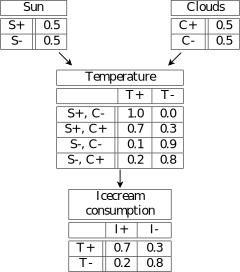
\includegraphics{images/graphical-model-example}
\par\end{centering}
\caption[Example of a graphical model.]{\label{fig:Example-of-a-graphical-model}Example of a graphical model. }
\end{figure}

\paragraph{Directed and Undirected Graphical Models}

In the following, we will introduce and discuss directed graphical
models and undirected graphical models. Directed graphical models
are also called \emph{Bayesian networks}\index{Bayesian network}
or \emph{Belief Networks}\index{Belief network}, and undirected graphical
models are also called \emph{Markov Random Fields}\index{Markov Random Field}
or \emph{Markov Networks}\index{Markov network}\footnote{There is also an unification of Bayesian networks and Markov random
fields, i.e. a graphical model that can have both directed and undirected
edges. These networks are called \emph{chain graphs} , or \emph{partially
directed acyclic graphs} and are not discussed here.}. We will consider only models with discrete random variable values.

\subsubsection{Undirected Graphical Models\label{par:Hammersley-Clifford-theorem}}

We want to encode a joint probability distribution $P$ in an undirected
graph $G=(\mathbf{N},\mathbf{E})$. Every random variable corresponds
to a node. The missing edges encode conditional independencies. A
complete graph would encode no conditional independencies. However,
we normally want to get a graph with the least possible edges (so
that the independencies between random variables in the joint probability
distribution are all represented in the graph). What properties does
the joint probability distribution $P$ have to fulfill so that it
can be encoded in an undirected graph and what does the minimal undirected
graph $G$ look like? This is answered by the \emph{Hammersley-Clifford
theorem}. \index{Hammersley-Clifford theorem} \cite{HammersleyClifford1971}

\paragraph{Hammersley-Clifford Theorem\label{par:The-Hammersley-Clifford-theorem-of-Undirected-Graphical-Model}}

Let $\mathbf{N}=\{N_{1},\dots,N_{n}\}$ be a vector of random variables,
$P(\mathbf{N})$ be a strictly positive joint probability distribution
with $P(\mathbf{n})>0$ for all possible values $\mathbf{n}$ of \textbf{$\mathbf{N}$},
and $G=(\mathbf{N},\mathbf{E})$ be an undirected graph with each
node corresponding to a random variable (i.e. $\mathbf{N}=\{N_{1},\dots,N_{n}\}$).
Then the following statements are equivalent:
\begin{itemize}
\item $P(\mathbf{N})$ factorizes according to the maximal cliques $\mathbf{C_{1}},\dots,\mathbf{C_{m}}$
in $G$, i.e. $P(\mathbf{N})=\frac{1}{Z}\phi_{1}(\mathbf{C_{1}})\cdot\ldots\cdot\phi_{m}(\mathbf{C_{m}})$,
where $Z$ is a scalar such that $\sum_{\mathbf{n}}P(\mathbf{N}=\mathbf{n})=1$,
i.e. $Z=\sum_{N_{1},\dots,N_{n}}\phi_{1}(\mathbf{C_{1}})\cdot\ldots\cdot\phi_{3}(\mathbf{C_{3}})$,
and the $\phi_{i}(\mathbf{C_{i}})$ depend only on the states of the
random variables in the clique $\mathbf{C_{i}}=(N_{i_{1}},\dots,N_{i_{n}})$
and must be positive for all possible states. $P(\mathbf{N})$ is
then called a \emph{Gibbs distribution}\index{Gibbs distribution},
$Z$ is called the \emph{partition function}\index{partition function},
and $\phi(\mathbf{C_{i}})$ are called the \emph{potential functions}\index{potential function}.
\item \label{local-Markov-property}the \emph{local Markov property}\index{local Markov property}
holds for the graph $G$ and the joint probability distribution $P$:
A node $N_{i}$ is conditionally independent from all non-neighbor
nodes $\mathbf{N}\backslash\mathbf{N_{neighbor(i)}}$, given the states
of the random variables $\mathbf{N_{neighbor(i)}}$ immediately connected
to $N$: $P(N_{i}\mid\mathbf{N_{neighbor(i)}})=P(N_{i}\mid\mathbf{N})$.
\item the \emph{global Markov property}\index{global Markov property} holds
for the graph $G$ and the joint probability distribution $P$: Given
any disjoint subsets $\mathbf{N_{A}},\mathbf{N_{B}},\mathbf{N_{S}}\subset\mathbf{N}$
where $\mathbf{N_{S}}$ separates the nodes $\mathbf{N_{A}}$ from
the nodes $\mathbf{N_{B}}$, and given the states of the random variables
of $\mathbf{N_{S}}$, the nodes $\mathbf{N_{A}}$ are conditionally
independent of the nodes $\mathbf{N_{B}}$: $P(\mathbf{N_{A}}\mid\mathbf{N_{S}})=P(\mathbf{N_{A}\mid}\mathbf{N_{S}},\mathbf{N_{B}})$.
\end{itemize}
Hence when we have a strictly positive joint probability distribution
$P(\mathbf{N})$, we can determine the corresponding minimal graph
$G$ with the following ``brute-force'' algorithm by using the local
Markov property: Start with the empty graph. For a variable $N_{i}$,
consider all sets of possible neighbor nodes, i.e. the power set $\mathbf{P}=\mathbb{\mathfrak{\mathcal{P}}}(\{\mathbf{N}\backslash N_{i}\})$,
and check for each such possible set of neighbors $\mathbf{N_{neighbors(i)}}$,
whether all non-neighbors $\mathbf{N_{nonneighbors(i)}}$ are independent
of $N_{i}$, given the neighbors
\[
N_{i}\,\mathbf{\,\indep\,\,N_{nonneighbors(i)}}\mid\mathbf{N_{neighbors(i)}},
\]
 i.e. whether $P(N_{i}\mid\mathbf{N_{neighbors(i)}},\mathbf{N_{nonneighbors(i)}})=P(N_{i}\mid\mathbf{N_{neighbors(i)}})$.
When a set of neighbors $\mathbf{N_{neighbors}}$ satisfying the conditional
independency has been found, we can draw an edge $E=(N_{i},N_{j})$
between $N_{i}$ and all neighbors $N_{j}\in\mathbf{N_{neighbors(i)}}$.
Repeat this for all variables $N_{i}\in\mathbf{N}$. Call the resulting
set of edges $\mathbf{E}$, and the minimal graph $G=(\mathbf{N},\mathbf{E})$.

On the other hand, if we have a graph $G=(\mathbf{N},\mathbf{E})$
consisting of a given set of nodes $\mathbf{N}$ and edges $\mathbf{E}$,
and local conditional probabilities $P(N\mid\mathbf{N}_{\mathbf{Parents}})$
at each node fulfilling the Markov property, then we can derive from
that the joint probability distribution over all random variables,
or equivalently over all nodes $\mathbf{N}$.

\paragraph{Example of an Undirected Graphical Model\label{par:Example-of-an-Undirected-Graphical-Model}}

\begin{figure}
\begin{centering}
\includegraphics[width=0.45\columnwidth]{images/undirected-graphical-model-example}
\par\end{centering}
\caption[Example of an Undirected Graph.]{\label{fig:Example-of-an-Undirected-Graph}Example of an Undirected
Graph encoding the following conditional independencies: the node
pairs (N1,N4), (N1,N5), (N2,N4), (N2,N5),(N4,N5) are conditionally
independent given node N3. (But (N1,N2) are not conditionally independent
given N3.)}
\end{figure}

For example, if there are the three cliques $\mathbf{C_{1}}=\{N_{1},N_{2},N_{3}\}$,
$\mathbf{C_{2}}=\{N_{3},N_{4}\}$, and $\mathbf{C_{3}}=\{N_{3},N_{5}\}$
(see figure \ref{fig:Example-of-an-Undirected-Graph}), then the joint
probability distribution $P$ (also called \index{Gibbs distribution}Gibbs
distribution) can be written as: 
\[
P(N_{1},\dots,N_{5})=\frac{1}{Z}\phi_{1}(\mathbf{C_{1}})\phi_{2}(\mathbf{C_{2}})\phi_{3}(\mathbf{C_{3}}),
\]
where $\phi_{1}(\mathbf{C_{1}})=\phi(N_{1},N_{2},N_{3})$ is the potential
function of clique 1 (\emph{clique potential}\index{clique potential}),
and is a function of the 3 random variables $N_{1},N_{2},N_{3}$ in
the clique. $Z$ is the partition function and must normalize the
function so that $P$ is a probability: 
\[
Z=\sum_{X_{1},\dots,X_{n}}\phi_{1}(\mathbf{C_{1}})\phi_{2}(\mathbf{C_{2}})\phi_{3}(\mathbf{C_{3}}).
\]

In practice, $\phi_{1}(N_{1},N_{2},N_{3})$ can be represented by
a table that holds, for each possible combination of states of the
three random variables, a positive real number. For example, if each
of the three random variables has two states, then the table (with
$2^{3}$ entries) could look like in table \ref{tab:Example-of-potential-function}.

\begin{center}
\begin{table}
\begin{centering}
\begin{tabular}{|c|c|c||c|}
\hline 
$n_{1}$ & $n_{2}$ & $n_{3}$ & $\phi(N_{1}=n_{1},N_{2}=n_{2},N_{3}=n_{3})$\tabularnewline
\hline 
\hline 
A & A & A & 0.124\tabularnewline
\hline 
A & A & B & 2.553\tabularnewline
\hline 
A & B & A & 0.842\tabularnewline
\hline 
$\vdots$ & $\vdots$ & $\vdots$ & $\vdots$\tabularnewline
\hline 
B & B & B & 1.258\tabularnewline
\hline 
\end{tabular}
\par\end{centering}
\caption{\label{tab:Example-of-potential-function}Example of a potential function
$\phi$ represented as a table.}
\end{table}
\par\end{center}

\subsubsection{Directed Graphical Models}

\begin{figure}
\begin{centering}
\includegraphics[width=0.3\columnwidth]{images/directed-graphical-model-example}
\par\end{centering}
\caption[Example of a Directed Graph.]{\label{fig:Example-of-a-Directed-Graph}Example of a Directed Graph.
Note that the graph is acyclic, and the nodes are laid out in layers.}
\end{figure}

Directed graphical models are also called \emph{Bayesian Networks}\index{Bayesian network}
or \emph{Belief Networks}\index{Belief network}. (See e.g. \cite{KollerTaskar2007,Neal1992}.)

Like undirected graphical models, directed graphical models represent
an implicit joint probability distribution over all random variables
present in the model. The graph must be directed and acyclic, and
each node of the graph is associated with a random variable. See figure
\ref{fig:Example-of-a-Directed-Graph} for an example.

A directed graphical model is defined by the directed graph $G=(\mathbf{N},\mathbf{E})$,
a prior probability distribution $P(N_{noparents})$ at the nodes
that do not have parents $\mathbf{N_{noparents}}$, and conditional
probability distributions $P(N_{hasparents}\mid\mathbf{N_{parents}})$
at the nodes that have parents $\mathbf{N_{hasparents}}$. In the
latter nodes the conditional probability distribution may only be
conditional on its immediate parents, not on distant ancestors. The
directed graph encodes the set of conditional independencies between
the random variables: A random variable $X$ of the graph is conditionally
independent of all random variables that are not descendants of $X$
(i.e. $\mathbf{N}\backslash\mathbf{N_{descendant(\mathbf{\mathrm{X}})}}$)
given the values of the parent variables of $X$ (this is called the
\emph{local Markov property}\index{local Markov property} of directed
graphs):
\[
X\,\,\indep\,\,(\mathbf{N}\backslash\mathbf{N_{descendant(\mathrm{X})}})\mid\mathbf{N_{parent(\mathrm{X})}}.
\]
(In general, independencies betweem any two sets of variables conditioned
on a third can be derived from the structure of the graph using \index{d-separation}\emph{d-separation}
\cite{Barber2012}.)

\paragraph{The Joint Probability Distribution Encoded by the Graphical Model\label{par:The-Joint-Encoded-by-Directed-Graphical-Model}}

In a directed graphical model, the random variables $\mathbf{N}$
can be totally ordered such that $N_{i}$ comes before $N_{j}$ if
there is a directed path from $N_{i}$ to $N_{j}$ in the graph, and
the order is unspecified if there is no directed path between $N_{i}$
and $N_{j}$ \cite{Neal1992}. (Thus, there are graphs which have
more than one compatible ordering, for example in the graph $A\rightarrow C\leftarrow B$,
the ordering can be $A,B,C$ as well as $B,A,C$.) In the following,
the ordering is expressed as the subscript $i\in\mathbb{N}$ of the
random variable $N_{i}$. The node $N_{i}$ has associated with it
the conditional probability $P(N_{i}=n_{i}\mid N_{j}=n_{j}\forall j<i)$.
(``The probability that the random variable $N_{i}$ is equal to
$n_{i}$ given that the random variables \textbf{$N_{j}$ }are equal
to $n_{j}$ where all subscripts $j$ that are smaller than $i$.'').

The joint probability distribution encoded by the graph is
\[
P(\mathbf{N})=P(N_{1}=n_{1},N_{2}=n_{2},\dots,N_{n}=n_{n})=\prod_{i=1}^{n}P(N_{i}=n_{i}\mid N_{j}=n_{j}\forall j<i).
\]

\paragraph{Example How to Represent the Conditional Probability Distribution}

For example, if the $N_{i}$ can only assume discrete $n_{i}$, the
conditional probability distribution can be represented by a table
with a size exponential in the number of involved nodes. When a node
has $a$ ancestors, each of which has $s$ possible states, and the
node itself also has $s$ possible states, then the table must contain
one probability for each of the $s^{a}\cdot(s-1)$ possible states.
($s^{a}$ for the combinations of the values of the ancestors and
$(s-1)$ for the values the node itself can assume.)

\subsection{Exact Inference in Graphical Models}

Inference in a graphical model is the task of answering a query about
the joint probability distribution encoded by the graph, or of a part
of the joint probability distribution. For example, one might be interested
in the overall probability of the configuration of a sub-set of variables.
However, in the general case this takes exponential time.

\subsubsection{Naive Approach: Marginalizing the Joint \label{par:Exact-Inference-in-Directed-and-Undirected Graphical Models}}

Since a graphical model is a representation of a joint probability
distribution, it can answer queries about probabilities of the joint
probability distribution encoded by the graphical model by first explicitly
calculating the joint, then marginalizing out non-interesting variables.

For example, we might want to infer the probability of a configuration
of variables when the values of only some of the variables are known.
We can then partition the variables $\mathbf{V}$ of a graphical model
into three disjoint groups:
\begin{enumerate}
\item the known variables $\mathbf{K}$,
\item the unknown variables $\mathbf{W}$ that we want to know the probability
distribution of,
\item the unknown variables $\mathbf{U}$ that we do not care about.
\end{enumerate}
Let the known values of $\mathbf{K}$ be written \textbf{$\mathbf{k}$}.
The unknown values of $\mathbf{W}$ are named \textbf{$\mathbf{w}$},
and the values of $\mathbf{U}$, $\mathbf{u}$. 

How to calculate the joint $P(\mathbf{W},\mathbf{U},\mathbf{K})$
encoded by the graphical model was defined in section \ref{par:The-Hammersley-Clifford-theorem-of-Undirected-Graphical-Model}
for undirected graphical models and in section \ref{par:The-Joint-Encoded-by-Directed-Graphical-Model}
for directed graphical models. Let's now turn our attention to marginalizing
out the non-interesting variables $\mathbf{U}$.

When we want to find the probability of configuration $\mathbf{W}=\mathbf{w}$,
given $\mathbf{K}=\mathbf{k}$, we can first write the query in terms
of the joint probability distribution. We have to condition on $\mathbf{K}$,
and marginalize out the unknown variables $\mathbf{U}$ that we do
not care about: 
\begin{eqnarray}
P(\mathbf{W}=\mathbf{w}|\mathbf{K}=\mathbf{k}) & = & \sum_{\mathbf{U}}P(\mathbf{W}=\mathbf{w},\mathbf{U}=\mathbf{u}|\mathbf{K}=\mathbf{k})\nonumber \\
 & = & \sum_{\mathbf{U}}\frac{P(\mathbf{W}=\mathbf{w},\mathbf{U}=\mathbf{u},\mathbf{K}=\mathbf{k})}{P(\mathbf{K}=\mathbf{k})}.\label{eq:Inference in graphical models}
\end{eqnarray}

In the above formula there is a sum over all variables \textbf{$\mathbf{U}$}.
Writing this out, we obtain 
\begin{eqnarray}
P(\mathbf{W}=\mathbf{w}|\mathbf{K}=\mathbf{k}) & = & \sum_{\mathbf{U}}\frac{P(\mathbf{W}=\mathbf{w},\mathbf{K}=\mathbf{k})}{P(\mathbf{K}=\mathbf{k})}\label{eq:Inference in graphical models, written out}\\
 & = & \sum_{U_{1}}\sum_{U_{2}}\cdots\sum_{U_{n}}\frac{P(\mathbf{W}=\mathbf{w},U_{1}=u_{1},U_{2}=u_{2},\dots,U_{n}=u_{n},\mathbf{K}=\mathbf{k})}{P(\mathbf{K}=\mathbf{k})}.\nonumber 
\end{eqnarray}

In the general case (if the joint probability cannot be factorized),
this nested sum needs $O(|\mathbf{u}|^{|\mathbf{U}|})=O(|\mathbf{u}|^{n})$
operations to compute, where $|\mathbf{u}|$ is the number of possible
values a variable $U_{i}$ can have (assuming for simplicity that
all random variables $U_{i}$ have the same number of possible values
$|\mathbf{u}|$) and $|\mathbf{U}|$ is the number of unknown variables
$U_{i}$. This is because all possible combinations of variable assignments
have to be considered. Thus, for this naive marginalization run-time
is exponential in the number of variables, and therefore intractable.

However, we have not yet considered the structure of the graph. We
can improve run-time in some cases of graphs and for some sets of
variables $\mathbf{K}$, $\mathbf{W}$, $\mathbf{U}$, as shown by
the following example.

\subsubsection{Factorization in Undirected Graphical Models}

In the case of an undirected graphical model, we can factorize the
joint probability into independent sub-joint-probabilities according
to the cliques. For instance, if the random variables $\mathbf{U}=\{U_{1},U_{2},\dots,U_{m}\}$
are composed of cliques $\mathbf{C_{1}},\mathbf{C_{2}},\dots,\mathbf{C_{n}}$,
so that $P(\mathbf{U})=\frac{1}{Z}\phi_{1}(\mathbf{C_{1}})\phi_{2}(\mathbf{C_{2}})\dots\phi_{n}(\mathbf{C_{n}})$,
then the above sum can be written, using Hammersley-Clifford, as
\begin{eqnarray*}
 & P(\mathbf{W}=\mathbf{w}|\mathbf{K}=\mathbf{k})\\
= & \sum_{U_{1}}\sum_{U_{2}}\cdots\sum_{U_{n}}\frac{P(\mathbf{W}=\mathbf{w},U_{1}=u_{1},U_{2}=u_{2},\dots,U_{n}=u_{n},\mathbf{K}=\mathbf{k})}{P(\mathbf{K}=\mathbf{k})}\\
= & \sum_{\mathbf{C}_{1}}\cdots\sum_{\mathbf{C}_{n}\backslash\{C_{1},\dots,C_{n-1}\}}\frac{\frac{1}{Z}\mbox{\ensuremath{\phi}}_{1}(\mathbf{W}=\mathbf{w},\mathbf{C}_{1}=\mathbf{c}_{1},\mathbf{K}=\mathbf{k})\cdot\ldots\cdot\mbox{\ensuremath{\phi}}_{n}(\mathbf{W}=\mathbf{w},\mathbf{C}_{n}=\mathbf{c}_{n},\mathbf{K}=\mathbf{k})}{P(\mathbf{K}=\mathbf{k})}\\
= & \frac{\frac{1}{Z}\left(\sum_{\mathbf{C}_{1}}\mbox{\ensuremath{\phi}}_{1}(\mathbf{W}=\mathbf{w},\mathbf{C}_{1}=\mathbf{c}_{1},\mathbf{K}=\mathbf{k})\cdot\left(\ldots\cdot\left(\sum_{\mathbf{C}_{n}\backslash\{C_{1},\dots,C_{n-1}\}}\mbox{\ensuremath{\phi}}_{n}(\mathbf{W}=\mathbf{w},\mathbf{C}_{n}=\mathbf{c}_{n},\mathbf{K}=\mathbf{k})\right)\right)\right)}{P(\mathbf{K}=\mathbf{k})}.
\end{eqnarray*}

The sums in the last line are nested sums that sum over all possible
states in the corresponding cluster. (If we order cliques descendingly
by the number of clique members then $\mathbf{C_{1}}$ is the largest
clique.) We still need to sum over the state combinations in the largest
clique. Therefore the run-time is at least $O(|\mathbf{u}|^{|\mathbf{C_{m}}|})$,
where $\mathbf{C_{m}}$ is the clique with the largest number of variables
in it. This is still an exponential run-time.


\subsubsection{Example of Inference in a Directed Graphical Model\label{subsec:Example-of-Exact-Inference-in-a-directed-graphical-model}}

Here we show an example how inference in a specific directed graphical
model is done. In our example, the directed graphical model is composed
of several densely connected layers, where the nodes within a layer
are not connected, and they have outgoing directed connections only
to nodes in the adjacent layer below.

When the probability distribution of the parent nodes are known, inferring
the probability distributions of child nodes is easy: just multiply
the probability of the parents with the conditional probability of
the child. To keep the example interesting, given the probability
distributions of the nodes in the bottom layer, we want to infer the
probability distributions for all the other nodes.

\paragraph{Deep Belief Networks}

For example consider the graph in figure \vref{fig:Example-of-a-Directed-Graph}.
This directed acyclic graph has the following directed connections
between its nodes: $G_{1}\rightarrow H_{1}$, $G_{1}\rightarrow H_{2}$,
$G_{2}\rightarrow H_{1}$, $G_{2}\rightarrow H_{2}$, $H_{1}\rightarrow V_{1}$,
$H_{1}\rightarrow V_{2}$, $H_{2}\rightarrow V_{1}$, $H_{2}\rightarrow V_{2}$.
Furthermore, the following conditional probability distributions are
given: $P(H_{1}|G_{1},G_{2})$, $P(H_{2}|G_{1},G_{2})$, $P(V_{1}|H_{1},H_{2})$,
$P(V_{2}|H_{1},H_{2})$. This layered architecture, where each node
in a layer is connected to all nodes in adjacent layers, defines a
directed graphical model called \emph{Deep Belief Network}\index{Deep Belief Network}.

\paragraph{Bayes Theorem Applied to Inference in a Deep Belief Network}

Now assume that $P(V_{1})$, $P(V_{2})$ are given and we want to
infer $P(G_{1}\mid\mathbf{V})$, $P(G_{2}\mid\mathbf{V})$, $P(H_{1}\mid\mathbf{V})$,
$P(H_{2}\mid\mathbf{V})$. Using Bayes' Theorem ($\mbox{posterior}=\mbox{likelihood}\cdot\mbox{prior}$)
we get
\begin{eqnarray}
P(H_{1},H_{2}|V,V_{2}) & = & \frac{P(V_{1},V_{2}|H_{1},H_{2})P(H_{1},H_{2})}{P(V_{1},V_{2})}\nonumber \\
 & = & \frac{P(V_{1},V_{2}|H_{1},H_{2})\left(\sum_{g_{1}}\sum_{g_{2}}P(g_{1})P(g_{2})P(H_{1}|g_{1},g_{2})P(H_{2}|g_{1},g_{2})\right)}{P(V_{1},V_{2})}\nonumber \\
 & = & \frac{1}{P(V_{1},V_{2})}\cdot P(V_{1}|H_{1},H_{2})P(V_{2}|H_{1},H_{2})\nonumber \\
 &  & \cdot\left(\sum_{g_{1}}\sum_{g_{2}}P(g_{1})P(g_{2})P(H_{1}|g_{1},g_{2})P(H_{2}|g_{1},g_{2})\right),\label{eq:deep-network-conditional-probability}
\end{eqnarray}
where 
\[
P(V_{1},V_{2})=\sum_{h_{1}}\sum_{h_{2}}P(V_{1}|H_{1}=h_{1},H_{2}=h_{2})P(V_{2}|H_{1}=h_{1},H_{2}=h_{2})P(H_{1}=h_{1},H_{2}=h_{2}).
\]
We can make the last transformation because $\ensuremath{V_{1}}$
and $\ensuremath{V_{2}}$ are independent given $\ensuremath{H_{1}},\ensuremath{H_{2}}$
(local Markov property). To determine $P(H_{1}|V_{1},V_{2})$ and
$P(H_{2}|V_{1},V_{2})$, we have to marginalize the other variable
in $\mathbf{H}$ out:
\begin{eqnarray}
P(H_{1}|V_{1},V_{2}) & = & \sum_{h_{2}}P(H_{1},H_{2}=h_{2}|V_{1},V_{2})\nonumber \\
P(H_{2}|V_{1},V_{2}) & = & \sum_{h_{1}}P(H_{1}=h_{1},H_{2}|V_{1},V_{2})\label{eq:deep-network-marginalization}
\end{eqnarray}

Since we now have $P(H_{1}|\mathbf{V})$, using $P(H_{1})=\sum_{v_{1}}\sum_{v_{2}}P(H_{1},V_{1}=v_{1},V_{2}=v_{2})$
and $P(H_{1}|V_{1},V_{2})=P(H_{1},V_{1},V_{2})/P(V_{1},V_{2})$ (and
equivalently $P(H_{1},V_{1},V_{2})=P(H_{1}|V_{1},V_{2})P(V_{1},V_{2})$),
we can determine $P(H_{1})$

\begin{eqnarray*}
P(H_{1}) & = & \sum_{v_{1}}\sum_{v_{2}}P(H_{1}|V_{1}=v_{1},V_{2}=v_{2})P(V_{1}=v_{1},V_{2}=v_{2}).
\end{eqnarray*}

$P(H_{2})$ can be computed similarly. Now that we know $P(H_{1})$
and $P(H_{2})$, we can repeat the steps to determine $P(G_{1}\mid\mathbf{H})$
and $P(G_{2}\mid\mathbf{H})$.

\subsubsection{Inference in Deep Belief Networks is Complicated\label{par:Exact-Inference-in-Deep-Belief-Networks-is-Complicated}}

The previous example shows that inference in a directed graphical
model with densely connected layers is complicated. If there are $n$
binary variables in $\mathbf{H}$ and $\mathbf{G}$, then the computation
of $P(\mathbf{H}\mid\mathbf{V})$ in equation \ref{eq:deep-network-marginalization}
takes $O(2^{n-1}n)$ due to having to marginalize out all variables
in $\mathbf{H}$ except one (the term $2^{n-1}$), and this for all
variables (the term $n$). In addition, this applies only if $P(\mathbf{H}\mid\mathbf{V})$
is known already. But in the computation of $P(\mathbf{H}\mid\mathbf{V})$,
equation \ref{eq:deep-network-conditional-probability}, there are
sums over the variables $g_{1}$ and $g_{2}$, which take another
$O(2^{n})$ in general. The phenomenon that leads to this computational
problem is called \emph{explaining away}\index{explaining away}.

The posterior of $H_{1}$ depends on all conditional probabilities
of the model, in this example, $P(\mathbf{V}\mid\mathbf{H})$ and
$P(\mathbf{H}\mid\mathbf{G})$. For Deep Belief Networks, which are
a kind of Directed Graphical Model with densely connected layers,
the conditional probabilities $P(\mathbf{V}\mid\mathbf{H})$ and $P(\mathbf{H}\mid\mathbf{G})$
have parameters called ``weights'' associated with them, and inference
of the layer immediately above $\mathbf{V}$, namely $\mathbf{H}$,
requires knowing all weights in the graph, not just those of $P(\mathbf{V}\mid\mathbf{H})$.
In addition, explaining away requires us to marginalize out all variables
in $\mathbf{H}$ except one, and this for all variables in $\mathbf{H}$.
A further problem is that we have to integrate over all variables
in all layers above $\mathbf{H}$ if we are interested in $P(\mathbf{H}\mid\mathbf{V})$.

These procedures become infeasible in a Belief Network with more than
a few parents per node. This is a problem in learning. If we want
to learn the parameters of a Deep Belief Network, we have to do inference.
However, we will see that there is a fast approximate learning algorithm.

\subsubsection{Intractability of Exact Inference on General Graphs}

Here we reference a proof by \cite{ChandrasekaranHarsha2012} that
low treewidth of the graph underlying inference in a graphical model
is the only structural property that enables tractable inference.

A \emph{triangulated graph}\index{triangulated graph} is a graph
where every loop having at least four nodes contains a \emph{chord}\index{chord},
i.e. an edge between two non-adjacent nodes in the loop\cite{Barber2012}.

For a triangulated graph, the \emph{treewidth}\index{treewidth} is
the number of nodes contained in the largest clique minus one. For
a graph of any form, the treewidth is the treewidth of the triangulation
that minimizes the treewidth. For directed acyclic graphs, the maximal
number of parents of any node is the critical number, since it determines
the treewidth of the moralized\footnote{You obtain a moralized graph from a directed acyclic graph by introducing
edges between all parents of a node, and then replacing directed edges
by undirected edges.} graph. (This was also shown by \cite{KwisthoutVanderGaag2010}.)

A graph is a \emph{minor}\index{minor of a graph}\emph{ }of a graph
$G$ if it is obtained from $G$ by one or more of the following operations:
1. deletion of an edge, 2. deletion of a node together with all edges
containing that node, and 3. contraction of an edge, which means an
edge $(N_{1},N_{2})$ and its two nodes $N_{1}$ and $N_{2}$ are
replaced with a new single node and the new node has edges to all
nodes that $N_{1}$ and $N_{2}$ had edges to.

Let $f(k)$ be the largest number such that every graph of treewidth
$k$ contains a grid of size $f(k)\times f(k)$ as minor. The \emph{grid-minor
hypothesis}\index{grid-minor hypothesis} states that $f(k)$ is polynomial
in $k$ (see \cite{ChandrasekaranHarsha2012}). \cite{ChekuriChuzhoy2014}
proved it in 2014.

A decision problem is in the complexity class $\mathbf{NP}$ if it
can be decided in time polynomial in the input by a non-deterministic
Turing machine. A decision problem is in the complexity class $\mathbf{P/Poly}$
if it can be decided in time polynomial in the input $x$ by a deterministic
Turing machine that receives as input not only $x$, but also an advice
string of length at most polynomial in the length of $x$ that may
only depend on the length of $x$, not $x$ itself\footnote{The advice string allows modeling pre-computation in the computation.}.
(See for example \cite{Sipser1996,Goldreich2008,AroraBarak2009}.)
The problem whether or not $\mathbf{NP}\subseteq\mathbf{P/Poly}$
is unsolved. 

\cite{ChandrasekaranHarsha2012} showed that under the assumptions
that the grid-minor hypothesis is true (which it is), and that $\mathbf{NP}\nsubseteq\mathbf{P/poly}$,
and given that arbitrary potential functions should be allowed, low
treewidth is the only structural property of otherwise arbitrary graphs
that ensures tractable run-time of exact inference on the graphical
model belonging to the graph. There exists no inference algorithm
with complexity polynomial in the treewidth.

If the assumption $\mathbf{NP}\nsubseteq\mathbf{P/poly}$ is correct,
then the only way to reduce the computational cost of exact inference
on a general graph with a given number of nodes is to reduce the
treewidth or to choose restricted potential functions (for example
constants) whose products do not require multiplication or can be
pre-computed. Therefore, in practice, the joint probability is approximated,
for example by Gibbs Sampling.

\subsection{Approximate Inference}

Approximate Inference in general graphical models by means of Gibbs
Sampling was first described by \cite{Neal1993}. We first have to
introduce Markov chains.

\subsubsection{Markov Chains}

For the following section, see e.g. \cite{Norris1997,GrinsteadSnell2003}
as references.


\paragraph{Markov property: Memorylessness}

A \emph{Markov chain}\index{Markov chain} is a sequence of random
variables $X_{t}$, where $t\in\mathbb{N}_{0}$ denotes the discrete
index of time. In a Markov chain, each random variable $X_{t}$ may
depend only on the state of the random variable at the immediate previous
time point $t-1$, i.e. 
\[
P(X_{t}=x_{t}\mid X_{0}=x_{0},\dots,X_{t-1}=x_{t-1})=P(X_{t}=x_{t}\mid X_{t-1}=x_{t-1})
\]
must hold for all $t\geq1$. This memorylessness is called the \emph{Markov
property}\index{Markov property}. In a Markov chain, possible states
$x_{t}$ at each time point are discrete and from the same set $\mathbb{S}$:
\begin{eqnarray*}
x_{t} & \in & \mathbb{S}\ \ \ \mbox{for all \ensuremath{t}}.
\end{eqnarray*}

\paragraph{Time-homogeneous Markov Chain and Transition Matrix}

A \emph{time-homogeneous Markov chain}\index{time-homogeneous Markov chain}
is a Markov chain in which the conditional probability $P(X_{t}=x_{t}|X_{t-1}=x_{t-1})$
is the same for all time points $t$, i.e. 
\[
P(X_{t}=x_{t}\mid X_{t-1}=x_{t-1})=P(X_{t-1}=x_{t-1}\mid X_{t-2}=x_{t-2})
\]
for all time points $t\geq2$. If this is the case, then this conditional
probability 
\[
P(X_{t}=j\mid X_{t-1}=i)\eqqcolon p_{ij}
\]
 is independent of the current time $t$ and can be written as the
matrix $p$, called the \emph{transition matrix}\index{transition matrix}.
In the following we will only deal with time-homogeneous Markov chains.

\paragraph{Computing future states from the initial distribution}

Let $d^{(t)}$ be the distribution of $X_{t}$, also named the \emph{probability
vector}\index{probability vector}, a row vector of length $|\mathbb{S}|$.
An entry $d_{i}^{(t)}$ is equal to the probability of $X_{t}$ having
state $x_{i}$: 
\begin{eqnarray*}
d_{i}^{(t)} & = & P(X_{t}=x_{i}).
\end{eqnarray*}
This implies $\sum_{i}d_{i}^{(t)}=1$ for all $t$. The distribution
$d^{(t+1)}$ can be computed from $d^{(t)}$ by matrix multiplication
with the transition matrix $p$: 
\[
d^{(t+1)}=d^{(t)}p.
\]
Given an initial distribution $d^{(0)}$ and the transition matrix
$p$, all $d^{(t)}$ are specified by 
\[
d^{(t)}=d^{(0)}p^{t}.
\]

\paragraph{Stationary distribution}

There are time-homogeneous Markov chains whose state distribution
stays constant once it has assumed a certain state distribution. Such
state distributions are called \emph{invariant}\index{invariant distribution}
or \emph{stationary distribution}\index{stationary distribution}.
A stationary distribution $\pi$ must fulfill the following equation:
\[
\pi p=\pi
\]
If $d^{(t)}=\pi$, then $d^{(t+u)}=\pi$ for all $u\geq0$. A Markov
chain can have more than one stationary distribution.

\paragraph{Detailed balance/Reversibility}

A Markov chain with transition matrix $p$ satisfies \emph{detailed
balance}\index{detailed balance}\emph{ }if there exists a probability
distribution $\pi=(\pi_{1},\pi_{2},\dots,\pi_{n})$ such that 
\[
\pi_{j}p_{ji}=\pi_{i}p_{ij}\ \ \ \mbox{for all \ensuremath{i}, \ensuremath{j}}.
\]
Such a Markov chain is also called a \emph{reversible} Markov chain\index{reversible Markov chain}
\cite{Norris1997}. A Markov chain with the detailed balance property
has at least one stationary distribution, where each stationary distribution
$\lambda$ fulfills the detailed balance condition: $\lambda_{j}p_{ji}=\lambda_{i}p_{ij}$
for all $i$, $j$.

While having detailed balance implies that a Markov chain has a stationary
distribution, the reverse is not true: there are Markov chains with
a stationary distribution but not satisfying detailed balance. For
example, a Markov chain with transition probabilities 
\[
(p_{ij})=\left(\begin{array}{ccc}
0 & 2/3 & 1/3\\
1/3 & 0 & 2/3\\
2/3 & 1/3 & 0
\end{array}\right)
\]
does not satisfy detailed balance, but $\pi=\left(\begin{array}{ccc}
\frac{1}{3} & \frac{1}{3} & \frac{1}{3}\end{array}\right)$ is a stationary distribution of this Markov chain \cite{Norris1997}.

\paragraph{Fundamental Theorem of Markov Chains\label{par:Fundamental-Theorem-of-Markov-Chains}}

Under what conditions does a Markov chain have an unique stationary
distribution? This is answered by the \emph{Fundamental Theorem of
Markov Chains}\index{fundamental theorem of Markov chains} \cite{Behrends2000}:

Theorem: Let $d^{(0)}$ and $e^{(0)}$ be any probability vectors
of a Markov chain with transition probabilities $(p_{ij})$, where
$(p_{ij})$ is irreducible, positive-recurrent and aperiodic. Then
the Markov chain converges to the unique stationary distribution $\pi$,
irrespective of the starting states:
\[
\lim_{t\rightarrow\infty}d^{(0)}p^{t}=\lim_{t\rightarrow\infty}e^{(0)}p^{t}=\pi.
\]

The definitions of irreducibility, positive recurrence, and aperiodicity
follow.

\paragraph{Irreducibility}

A Markov chain is called \emph{irreducible}\index{irreducible}, if
it is possible to go from any state $i$ of the Markov chain to any
state $j$ (possibly in more than 1 steps). Formally, a Markov chain
is called irreducible, if its states are all in the same (and only)
closed subset. A subset $C$ of $\mathbb{S}$ is called \emph{closed
}if $p_{ij}=0$ whenever $i\in C$ and $j\notin C$. (Remember that
$\mathbb{S}$ is the set of possible states of the Markov chain.)

\paragraph{Positive Recurrence}

A state $i$ of a Markov chain is \emph{positive recurrent}\index{positive recurrent},
if we expect the Markov chain to take a finite number of steps until
it is in state $i$ again, when it started in state $i$ at time point
$0$. To define positive recurrence formally, we have to define auxiliary
measures first. The probability that state $j$ is visited at time
step $k$ for the first time after the Markov chain had been in state
$i$ at time point $0$ is 
\[
f_{ij}^{(k)}:=P(X_{1}\neq j,X_{2}\neq j,\dots,X_{k-1}\neq j,X_{k}=j\mid X_{0}=i).
\]
The probability that state $j$ is ever reached from state $i$ is
\[
f_{ij}^{*}:=\sum_{k=1}^{\infty}f_{ij}^{(k)}.
\]
With this, we can define the expected number of steps for the Markov
chain to reach state $j$, when starting at state $i$:
\[
\mu_{ij}:=\sum_{k=1}^{\infty}kf_{ij}^{(k)}.
\]
This number is also called the \emph{mean recurrence time}\index{mean recurrence time}.
With these definitions, we can define a state to be \emph{transient}\index{transient},
positive recurrent, or \emph{null recurrent}\index{null recurrent}:
\begin{itemize}
\item If $f_{ii}^{*}<1$, the state $i$ is called transient.
\item If $f_{ii}^{*}=1$, the state $i$ is called recurrent.

\begin{itemize}
\item If $f_{ii}^{*}=1$ and $\mu_{ii}<\infty$, the state $i$ is called
\emph{positive recurrent}.
\item If $f_{ii}^{*}=1$ and $\mu_{ii}=\infty$, the state $i$ is called
\emph{null recurrent}.
\end{itemize}
\end{itemize}
It can be proven that when there are finitely many states, there are
no null recurrent states (see Proposition 7.2. in \cite{Behrends2000}).

\paragraph{Aperiodicity}

The definition of an \emph{aperiodic}\index{aperiodic} state is shorter.
The period of a state\index{period of a state} $i$ is defined as
the greatest common denominator of the number of time steps needed
for a Markov chain so that it is possible to be in state $i$ again,
after it was in state $i$ before: 
\[
period(i)=gcd(\{k\mid k\geq0,(p^{k})_{ii}>0\}).
\]
If $period(i)=1$, state $i$ is called \emph{aperiodic}. If all states
of a Markov chain are aperiodic, the Markov chain is called aperiodic.

\paragraph{Markov Chain Monte Carlo (MCMC)}

\emph{Markov Chain Monte Carlo}\index{Markov Chain Monte Carlo algorithm}\index{MCMC algorithm}
is an algorithm to sample from a multivariate probability distribution.
It sets up a Markov chain that converges to the desired stationary
distribution and iterates it through time until the stationary distribution
is approximated sufficiently.

A trick can be useful. To efficiently calculate the stationary distribution
$\pi$, compute only the transition matrix for time steps that are
a power of 2, i.e. $p^{2^{t}}$. This can be done by starting with
$p^{1}:=p$, repeated squaring: $p^{2t}:=p^{t}p^{t}$, and assigning
the stationary distribution $\pi=d^{(0)}p^{2^{t}}$ for a large enough
$t$.

MCMC will be described in the next section. 

\subsubsection{Gibbs Sampling}

Here, we will review Gibbs Sampling to show how \cite{Neal1993} used
it to approximate inference in directed and undirected graphical models.

\emph{Gibbs Sampling}\index{Gibbs sampling} \cite{GemanGeman1984}
is an instance of a Markov chain Monte Carlo (MCMC) algorithm. Its
goal is to generate samples from a multivariate joint probability
distribution, without having to know its closed form. The generated
samples can then be used to compute an approximation of the mean of
a distribution, for example.

To use a Gibbs Sampler, one must construct a Markov chain with its
(only) stationary distribution equal to the target distribution. Each
random variable is updated in turn, based on the conditional probabilities.

\paragraph{Gibbs Sampling Requires Closed-form Conditional Probabilities}

Suppose that the multivariate target distribution is $P(X_{1},\dots,X_{n})$.
Here, for each random variable $X_{i}\in\{X_{1},\dots,X_{n}\}$, the
conditional probability of the variable given all other variables
must be known in closed form, so that it can be evaluated: 
\[
P(X_{i}\mid\mathbf{X_{j}},j\in\{1,\dots,n\}\backslash i)=P(X_{i}\mid X_{1},\dots,X_{i-1},X_{i+1},X_{n}).
\]
Another prerequisite is that Gibbs Sampling, which requires sampling
from the conditional probability distribution and iterating, should
be faster than sampling from the joint target probability distribution
directly.

\paragraph{A Markov Chain in Multiple Dimensions}

The variable updates in Gibbs Sampling can be regarded as a Markov
chain. However, we must first define how the random variables of Gibbs
Sampling are mapped to the random variable of the Markov chain. One
possibility is to re-map the random variables and their states to
a single random variable.

Above, Markov chains were defined for a single state variable $X$.
But in Gibbs Sampling there are usually more than one variable, written
$X_{i}\in\{X_{1},\dots,X_{n}\}$ above. If there are a finite number
of random variables in Gibbs Sampling, and the state space of these
variables is also finite, say of size $m$, then the (therefore also
finite) number of states of these variables can be encoded in a single
variable with a state space of size $m^{n}$.

For example, say there are 3 variables, each of which can assume 2
states, and we want to encode these $2^{3}$ different possible states
in one variable. Then the Markov chain has one variable with $2*2*2$
different possible states.

\paragraph{Constructing a Markov Chain from Base Transitions}

\cite{Neal1993} suggests constructing a non-homogeneous Markov
chain with transition matrix $T$ by applying base transitions in
turn, each of which describe the probability of a state change of
one random variable. The base transitions are named $B_{k}(x,x')$,
where $k\in1,2,\ldots,s$ is the index of the base transition, $x$
is the starting state of the transition, $x'$ is the target state
of the transition. $B_{k}(x,x')$ is the probability of the transition
and must be strictly greater than zero for all values of $x$ and
$x'$, to make the Markov chain irreducible. At each time-point $a*s+k-1$
with $a\in\mathbf{\mathbb{N}}$, the next single base transition $B_{k}(x,x')$
is then applied:

\[
T_{as+k-1}(x,x')=B_{k}(x,x').
\]

\cite{Neal1993} also notes that the required properties for a Markov
chain to converge are fulfilled: If each of the base transitions $B_{k}$
have a stationary distribution, then the non-homogeneous $T$ also
has a stationary distribution.

\paragraph{Initialization of the Gibbs Sampler}

A Gibbs Sampler starts by specifying a start value $x_{i}^{(0)}$
for each random variable $X_{i}$. Since the Markov chain must be
constructed such that it converges to its only stationary distribution
the choice of start values is not critical, but it influences the
numbers of iterations needed until the Gibbs Sampler returns samples
from the target distribution. So the start value should be close to
the expected value of the distribution.

\paragraph{Iterating}

Then an iterative process is started. In each iteration $t$, each
random variable $X_{i}$ is updated by sampling a new value $x_{i}^{(t)}$
from the conditional probability distribution 
\begin{equation}
P(X_{i}\mid X_{1}=x_{1}^{(t-1)},\dots,X_{i-1}=x_{i-1}^{(t-1)},X_{i+1}=x_{i+1}^{(t-1)},\dots,X_{n}=x_{n}^{(t-1)}).\label{eq:Gibbs sampling: CPD}
\end{equation}

There are different alternative ways in which the random variables
are updated, for example updating the random variables can be done
in random order, or sequentially, or a whole ``block'' of multiple
random variables can be sampled from the conditional distribution
given all the other random variables (e.g. $P(X_{i_{1}},X_{i_{2}},X_{i_{3}}\mid\mathbf{X_{j}=x_{j}^{(t-1)}},j\in\{1,\dots,n\}\backslash\{i_{1},i_{2},i_{3}\})$).

If the Markov chain fulfills irreducibility, positive recurrence,
and aperiodicity, then it is guaranteed to converge to its stationary
distribution (Fundamental Theorem of Markov Chains). However there
is currently no known analytic method to determine when the Markov
chain has reached its stationary distribution, which leads to the
following two strategies, \emph{burn-in} and \emph{thinning}.

\paragraph{Burn-in Period}

The starting value of the random variable might be far from the ``center''
of the distribution. But after some number of throw-away iterations,
the Gibbs Sampler's values $\mathbf{x}=(x_{1},\dots,x_{n})$ will
start coming from the target joint distribution $P(X_{1},\dots,X_{n})$.
This ``some number of throw-away iterations'' is called the \emph{burn-in
period}\index{burn-in period} and can be considerable depending on
the starting values and the joint probability distribution underlying
the conditional probability distributions. If one knows where the
``center'' of the equilibrium distribution is then one should use
a value near that center as the starting point, however, in many cases
such things are not known (and may be the goal of Gibbs Sampling in
the first place).

There is no known analytic method to determine when a chain is burned-in.
Several convergence diagnostics methods have been proposed, see e.g.
\cite{CowlesCarlin1996} for a review.

\paragraph{Thinning}

\index{thinning}Even after the Markov chain is burned in, there is
still a problem with the returned samples, which prevent them from
being used in those applications needing \emph{independent }samples.
The samples of two adjacent time steps $\mathbf{x}^{(t)}$ and $\mathbf{x}^{(t+1)}$
are correlated however, because the latter is dependent on the former
(by definition).

This can be mitigated by returning only the states of every $n$th
iteration, where $n$ is a sufficiently large number. This is called
``thinning'' of the Gibbs sampler.

Again, there is currently no straightforward analytic way to determine
what a sufficiently large $n$ is for the adjacent $\mathbf{x}$ to
be regarded independent. In practice one resorts to heuristics like
autocorrelation.

\subsubsection{Gibbs Sampling in Markov Random Fields and Bayesian Networks \label{subsec:Inference-in-Markov-Random-Fields}}

We can now define the algorithms for approximate inference using Gibbs
Sampling in Markov Random Fields and Bayesian Networks.

In Markov Random Fields, we use the local Markov property: each random
variable $X_{i}$ is independent of all other random variables given
the states of the neighboring random variables. Thus, in Markov Random
Fields, the conditional probability (see equation \ref{eq:Gibbs sampling: CPD})
is 
\[
P(X_{i}\mid X_{1},\dots,X_{i-1},X_{i+1},\dots,X_{n})=P(X_{i}\mid\mathbf{X}_{Neighborhood(X_{i})}).
\]
In Bayesian Networks the conditional probability is 
\[
P(X_{i}\mid X_{1},\dots,X_{i-1},X_{i+1},\dots,X_{n})=P(X_{i}\mid\mathbf{X}_{MarkovBlanket(X_{i})}),
\]
where $\mathbf{X}_{MarkovBlanket(X_{i})}$ are the random variables
in the Markov Blanket of $X_{i}$.

\paragraph{Gibbs Sampling in Markov Random Fields\label{par:Gibbs-Sampling-in-Markov-Random-Fields}}

Exact inference in Markov Random Fields can be done by conditioning
on the known random variables and marginalizing out the uninteresting
variables (see section \ref{par:Exact-Inference-in-Directed-and-Undirected Graphical Models}).
The exponential runtime of exact inference can be circumvented by
approximate methods like Gibbs Sampling.

For example, we might want to infer the probability of a configuration
of variables when the values of only some of the variables are known.
We can partition the variables $\mathbf{X}:=\mathbf{U}\cup\mathbf{K}\cup\mathbf{W}$
of a graphical model into three disjoint groups:
\begin{enumerate}
\item the variables $\mathbf{K}$ whose states are known (for example because
they were measured)
\item the unknown variables $\mathbf{W}$ that we want to know the probability
distribution of,
\item the unknown variables $\mathbf{U}$ that we do not care about.
\end{enumerate}
Gibbs Sampling in Markov Random Fields uses a converging Markov chain
to sample from the target joint probability distribution. A prerequisite
is that the conditional probability distributions are known in closed
form.
\begin{enumerate}
\item Initialize the state $x_{i}^{(1)}$ of the random variable $X_{i}\in\mathbf{W}\cup\mathbf{U}$
with an arbitrary state.
\item Initialize the state $x_{i}^{(1)}$ of the known random variables
$X_{i}\in\mathbf{K}$ with their known state.
\item \label{enu:For-each-time}For each time point $t\in\{1,2,\dots\}$
do

\begin{enumerate}
\item Keep the known variables fixed (i.e. $x_{i}^{(t+1)}:=x_{i}^{(t)}$
for all $X_{i}\in\mathbf{K}$).
\item For each random variable $X_{i}\in\mathbf{W}\cup\mathbf{U}$ do

\begin{enumerate}
\item Given the states of all variables $\mathbf{X}\backslash X_{i}$, sample
a new $X_{i}$ from its conditional distribution $P(X_{i}=x_{i}^{(t+1)}\mid X_{1}=x_{1}^{(t)},\dots,X_{i-1}=x_{i-1}^{(t)},X_{i+1}=x_{i+1}^{(t)},\dots,X_{n}=x_{n}^{(t)})$.
The Hammersley-Clifford theorem  states that this conditional probability
is equal to $P(X_{i}=x_{i}^{(t+1)}\mid\mathbf{X}_{Neighborhood(X_{i})})$.
\end{enumerate}
\end{enumerate}
\item Repeat step \ref{enu:For-each-time} until the Markov chain converges.
\item Discard the states of the uninteresting random variables $\mathbf{U}$.
\item Return the states of the interesting random variables $\mathbf{W}$.
\end{enumerate}

\paragraph{Gibbs Sampling in Bayesian Networks}

We use the same algorithmic structure as for Markov Random Fields
above, but sample from a different conditional probability distribution
$P(X_{i}=x_{i}\mid\mathbf{X_{j}}=\mathbf{x_{j}}:j\neq i)$ when updating
the state of $X_{i}$ in step \ref{enu:For-each-time}(b).

The conditional probability of $X_{i}$ given all other nodes is equal
to its conditional probability given the values of the nodes in $X_{i}$'s
Markov Blanket $X_{MarkovBlanket(X_{i})}$
\[
P(X_{i}=x_{i}\mid\mathbf{X_{j}}=\mathbf{x_{j}}:j\neq i)=P(X_{i}=x_{i}\mid\mathbf{X}_{MarkovBlanket(X_{i})}=\mathbf{x}_{MarkovBlanket(X_{i})}),
\]
where $\mathbf{X}_{MarkovBlanket(X_{i})}$ is the set of $X_{i}$'s
parents and children, and its children's parents. Formally, and parallel
to section 4.1 in \cite{Neal1993}, the conditional probability distribution
$P(X_{i}=x_{i}\mid\mathbf{X}_{MarkovBlanket(X_{i})})$ is equal to
\begin{eqnarray*}
P(x_{i}\mid\{x_{i}:i\neq k\}) & = & P(x_{i}\mid\mathbf{x}_{MarkovBlanket(X_{i})})\\
 & = & \frac{P(x_{i}\mid\mathbf{x}_{Parent(i)})\prod_{j\in Child(i)}P(x_{j}\mid x_{i},\mathbf{x}_{Parent(j)\backslash i})}{\sum_{\tilde{x}_{i}}P(\tilde{x}_{i}\mid\mathbf{x}_{Parent(i)})\prod_{j\in Child(i)}P(x_{j}\mid\tilde{x}_{i},\mathbf{x}_{Parent(j)\backslash i})}.
\end{eqnarray*}

\section{Artificial Neural Networks}

Here we will introduce artificial neural networks that have been developed
as models of biological neural networks since in the middle of the
last century. The artificial neural networks introduced here are related
to Deep Belief Networks, namely Hopfield networks, Multilayer Perceptrons,
and (Restricted) Boltzmann Machines.

\paragraph{Distinction Between a Deterministic and Stochastic Network}

In a deterministic network\index{deterministic network} a node represents
a deterministic value. In contrast, in a stochastic network\index{stochastic network}
a node represents a probability distribution. If there is a set of
``output'' nodes, then in a deterministic setting the output can
be interpreted as a point in a high-dimensional space, while in a
stochastic network the output is the joint probability distribution
over all the random variables associated with the output nodes.

A stochastic network is more general than its deterministic counterpart,
since a stochastic network can be converted to a deterministic network,
but not vice-versa. This comes at a higher cost. Inference and learning
in stochastic networks take longer than in deterministic networks.

\paragraph{Distinction Between Feed-forward and Recurrent Networks}

A \emph{feed-forward network}\index{feed-forward neural network}\emph{
}is a network defined on a directed acyclic graph. In contrast, the
connections of a \emph{recurrent network}\index{recurrent neural network}\emph{
}may form cycles.

\subsection{Hopfield Networks}

\paragraph{Structure}

A \emph{Hopfield Network}\index{Hopfield Network} \cite{Hopfield1984}
is a deterministic recurrent network with $m$ nodes, each having
a binary state $n_{i}\in\{0,1\}$ for all nodes $i$. Every node is
connected with all others but not with itself. The connection from
node $N_{i}$ to node $N_{j}$ is directed and has a weight $w_{ij}\in\mathbb{R}$.
There is no self-connection from node $i$ to node $i$, and therefore
$w_{ii}=0$ for all nodes $i$. Hence, each node has $m-1$ outgoing
connections and $m-1$ incoming connections. There is also a real-valued
bias $b_{i}\in\mathbb{R}$ for each node $i$ that acts as a weight
of a connection from a ``virtual'' node that always has state 1.
Figure \ref{fig:Example-of-a-Hopfield-Network} shows an example of
the structure of a Hopfield Network.

\begin{figure}
\begin{centering}
\includegraphics[width=0.3\columnwidth]{images/hopfield-network-example}
\par\end{centering}
\caption[Example of a Hopfield Network.]{\label{fig:Example-of-a-Hopfield-Network}Example of a Hopfield Network.
The circles are the nodes; the arrows are the (directed) connections.}
\end{figure}

\paragraph{Associative Memory}

Hopfield networks can be used as \emph{associative }or\emph{ content-addressable
memory}\index{associative memory}\index{content-addressable memory},
where the memory is a binary number. Bit $i$ of the memory is stored
in node $i$ of the network. Associative or content-addressable memory
means that the network can be initialized with a partially distorted
memory and the network can recall a previously learned memory that
is close to the initialized memory. Recalling a partially known memory
is done by repeatedly updating the network.

\paragraph{Updating Rule}

The network is updated asynchronously: At each time point $t$, a
node $i$ is chosen at random out of the $m$ possible nodes and it
is updated, while all other nodes remain constant. The state $n_{i}$
of node $i$ at time point $t$ is denoted $n_{i}^{(t)}$ and depends
on the state of all other nodes at time step $t-1$, the weights $w_{ji}$
from node $j$ to node $i$, and the bias $b_{i}$: 
\[
n_{i}^{(t)}=f\left(\sum_{j\neq i}n_{j}^{(t-1)}w_{ji}+b_{i}\right),
\]
where the \emph{activation function}\index{activation function} $f$
is a step function that maps nonpositive values to 0, and positive
values to 1: 
\[
f(x)=\begin{cases}
0 & \mbox{for }x\leq0\\
1 & \mbox{for }x>0
\end{cases}.
\]
(In \cite{Hopfield1984} there is also an external input to each
node, constant over all times $t$. Because the bias also does not
depend on $t$, both are combined into $b_{i}$ here.)\\
As described here, the updating rule is asynchronous (i.e. at each
time step a node is picked at random and its state is updated, which
is how Hopfield described it \cite{Hopfield1984}). Updating the
network synchronously (i.e. all nodes are updated at the same time)
is also possible.

\paragraph{Energy of a Hopfield Network}

The \emph{energy }\index{energy} is associated with the state of
the network at time point $t$ and is defined as

\begin{equation}
E^{(t)}=-\frac{1}{2}\sum_{i}\sum_{j\neq i}w_{ij}n_{i}^{(t)}n_{j}^{(t)}-\sum_{i}b_{i}n_{i}^{(t)}.\label{eq:Energy of a Hopfield network}
\end{equation}
Hopfield showed that when applying the updating rule repeatedly, the
energy converges to a (possibly local) minimum, provided that the
weights are symmetric (i.e. $w_{ij}=w_{ji}$) and there are no single-node
loops (i.e. $w_{ii}=0$). In more detail, each update of a node either
doesn't change the energy $E$ or decreases it. As time progresses
$E$ becomes smaller and smaller, i.e. $E^{(t)}\leq E^{(t-1)}$.


\paragraph{Recalling a Training Pattern by the Updating Rule}

Training a Hopfield network is the task of finding weights $w_{ij}$
and biases $b_{i}$, so that training patterns (i.e. memories to be
learned) have a low energy and all other states have a high energy.
After training, a Hopfield network can be initialized with a distorted
pattern, in which the states of some nodes are inverted. After iteratively
updating the network until its state doesn't change anymore, the stationary
state will be similar to a training pattern. In a demonstration of
\cite{Hopfield1982}, approximately 85\% of the trials ended in training
patterns, 5\% resulted in stable states near training patterns, and
10\% ended in stable states of no obvious meaning.

\subsection{Multilayer Perceptrons}

\paragraph{Structure}

A Multilayer Perceptron belongs to the class of deterministic feed-forward
neural networks. The neurons are arranged in layers, with the value
of nodes in a layer only depending on the values of nodes in the layer
above. Example structures of multilayer perceptrons were given in
figure \vref{fig:sigmoid-function} and figure \vref{fig:Data-flow-in-back-propagation}.

\subsubsection{Multilayer Feed-forward Networks as Universal Function Approximators}

\cite{HornikWhite1989} found that artificial feed-forward neural
networks with as few as one hidden layer can model any Borel measurable
function within a given error, provided the following conditions are
met:

\pagebreak{}
\begin{itemize}
\item The activation function must be a ``squashing'' function: A squashing
function $s(x)$ must be non-decreasing, $\lim_{x\rightarrow-\infty}s(x)=0$
and $\lim_{x\rightarrow\infty}s(x)=1$. An example is the sigmoid
function $\frac{1}{1+exp(-x)}$.
\item Sufficiently many hidden nodes must be available.
\end{itemize}
\cite{HornikWhite1989} also note that ``This {[}result{]} implies
that any lack of success in applications must arise from inadequate
learning, insufficient numbers of hidden units{[}nodes{]} or the lack
of a deterministic relationship between input and target.''

\subsubsection{Training Using Back-propagation}

\emph{Back-propagation}\index{back-propagation} is the adaptation
of weights and biases of the network to make its set of actual outputs
better fit a set of desired outputs for a given set of inputs. Technically
it is just running the network for a given input in the forward pass\index{forward pass},
observing the outputs in the output layer, computing the errors to
the desired outputs and back-propagating them to adapt the weights
and biases between all the layers. This will make the network output
values closer to the desired values next time this particular input
pattern is given to the network. The back-propagation algorithm is
a supervised learning step and thus prone to overfitting. In order
to discuss modifications and extensions of the algorithm, we will
first repeat the most important points of back-propagation as reviewed
in section \ref{subsec:Back-propagation}.

\paragraph{Forward and Backward Pass}

In the \emph{forward pass}\index{forward pass}, each node's output
is computed from the sum of its inputs
\begin{eqnarray*}
v_{j} & = & b_{j}+\sum_{i\in\mathbf{c_{j}}}o_{i}w_{ji},
\end{eqnarray*}
 where $b_{j}$ is the bias, $o_{i}$ is the output of a node in the
layer above, and $w_{ji}$ is the weight of the connection from node
$i$ to node $j$. The input $v_{j}$ is then scaled by the sigmoid
function to produce a node's output $o_{j}$

\[
o_{j}=\sigma(v_{j})=\frac{1}{1+\exp(-v_{j})}.
\]

In the \emph{backward pass}\index{backward pass}, the training procedure
computes the total error $E$ of the network, which is defined as
the squared sum of differences between actual output $o_{k}$ and
desired output $y_{k}$
\[
E=\frac{1}{2}\sum_{k}(o_{k}-y_{k})^{2},
\]
 where $o_{k}$ is the actual activation of node $k$ in the output
layer, and $y_{k}$ is its desired output. The sum-of-squared-differences
term $\frac{1}{2}\sum_{k}(o_{k}-y_{k})^{2}$ is called the \emph{error}\index{error function},\emph{
loss }\index{loss function}, or \emph{cost} function\index{cost function}.

\paragraph{Error of the Output Layer}

The error is then differentiated with respect to a weight $w_{kj}$
for a connection from node  $j$ in the last hidden layer to node
$k$ in the output layer 
\begin{equation}
\frac{\partial E}{\partial w_{kj}}=\frac{\partial E}{\partial o_{k}}\cdot\frac{\partial o_{k}}{\partial v_{k}}\cdot\frac{\partial v_{k}}{\partial w_{kj}}=(o_{k}-y_{k})\cdot o_{k}(1-o_{k})\cdot o_{j},\label{eq:backpropagation-error-wrt-weight}
\end{equation}
 and with respect to $b_{k}$
\[
\frac{\partial E}{\partial b_{k}}=\frac{\partial E}{\partial o_{k}}\cdot\frac{\partial o_{k}}{\partial v_{k}}\cdot\frac{\partial v_{k}}{\partial b_{k}}=(o_{k}-y_{k})\cdot o_{k}(1-o_{k})\cdot1.
\]

\paragraph{Error of the Other Layers}

The derivative of the error with respect to the weights $w_{ji}$
of the remaining connections from node $i$ in a layer to node $j$
in the layer below is
\begin{eqnarray*}
\frac{\partial E}{\partial w_{ji}} & = & \frac{\partial E}{\partial o_{j}}\cdot\frac{\partial o_{j}}{\partial v_{i}}\cdot\frac{\partial v_{i}}{\partial w_{ji}}\\
 & = & \frac{\partial E}{\partial o_{j}}\cdot o_{j}(1-o_{j})\cdot o_{i},
\end{eqnarray*}
 where
\begin{eqnarray*}
\frac{\partial E}{\partial o_{j}} & = & \sum_{k}\frac{\partial E}{\partial o_{k}}\frac{\partial o_{k}}{\partial v_{k}}w_{kj}
\end{eqnarray*}
and we take the value for $\frac{\partial E}{\partial o_{k}}\frac{\partial o_{k}}{\partial v_{k}}$
from node $k$, which is in the layer below node $j$. Analogously,
the derivative with respect to $b_{j}$ is 
\begin{eqnarray*}
\frac{\partial E}{\partial b_{j}} & = & \sum_{k}\frac{\partial E_{k}}{\partial o_{k}}\frac{\partial o_{k}}{\partial v_{k}}w_{kj}\cdot o_{j}(1-o_{j})\cdot1.
\end{eqnarray*}

\paragraph{Updating Rule and Learning Rate}

After computing the derivatives of the error with respect to the parameters
of the network, we can perform gradient descent and update the parameters
using the learning rate\index{learning rate} $\epsilon$, a small
positive number:
\begin{eqnarray}
\Delta w & = & -\epsilon\frac{\partial E}{\partial w}\label{eq:backpropagation-deltas}\\
\Delta b & = & -\epsilon\frac{\partial E}{\partial b}.\nonumber 
\end{eqnarray}

\paragraph{Optimizing the Sum of Squared Differences Error\label{par:Optimizing-the-Sum-of-Squared-DIfferences}}

Usually in back-propagation, the error function to be minimized is
the \emph{sum of squared differences}\index{sum of squared errors}\index{squared-error sum}
between the desired outputs and the actual outputs
\[
E=\frac{1}{2}\sum_{k}(o_{k}-y_{k})^{2},
\]
 where $y_{k}$ is the desired value of node $k$ in the output layer
and $o_{k}$ is the actual output value of node $i$. As stated in
equation \ref{eq:backpropagation-error-wrt-weight}, the derivative
of the error $E$ with respect to a weight $w_{kj}$ is
\begin{equation}
\frac{\partial E}{\partial w_{kj}}=(o_{k}-y_{k})\cdot o_{k}(1-o_{k})\cdot o_{j}.\label{eq:backpropagation-error-wrt-weight-1}
\end{equation}

\paragraph{Optimizing the Cross-entropy Error\label{par:Optimizing-the-Cross-entropy-error}}

Another error function is the \emph{cross-entropy error}\index{cross-entropy error}
\cite{NasrJoun2002} 
\[
E=-\sum_{k}y_{k}\log o_{k}-\sum_{k}(1-y_{k})\log(1-o_{k}),
\]
 where again $y_{k}$ is the desired output value of node $k$ in
the output layer and $o_{k}$ is the actual output value. The derivative
of error $E$ with respect to a weight $w_{kj}$ from node $j$ in
the last hidden layer to node $k$ in the output layer is then
\[
\frac{\partial E}{\partial w_{kj}}=(o_{k}-y_{k})o_{j}.
\]

\cite{GolikNey2013} note that using the cross-entropy error function
requires less updates, since the gradient for the sum-of-squared-differences
error function becomes low not only when the actual output $o_{k}$
is near the desired output $y_{k}$, but also when $o_{k}$ is near
0 or 1 (see equation \ref{eq:backpropagation-error-wrt-weight-1}).

\subsubsection{Parameters in Training a Neural Network\label{subsec:Parameters-of-Training-a-Multilayer-Perceptron}}

Although described here for multilayer perceptrons, the parameters
apply to most artificial neural networks, not just multilayer perceptrons.

\paragraph{Random Weight and Bias Initialization}

At the start of training, weights $w$ and biases $b$ have to be
initialized. They must not all be initialized to the same value, because
then the activations in the output layer $o_{k}$ would become equal,
leading to an equal error gradient for the weights and biases, which
would prevent learning. Ideally, the hidden and output layer activations
$o_{j}$ should be in the linear region of the activation function,
so that the error derivatives are large. As \cite{LeCunMuller1998}
note, this requires coordinating the training set  normalization,
the choice of the activation function, and the weight and bias initialization.

Usually the biases are initialized to zero, and the weights are drawn
from a uniform random distribution in {[}-1;1{]}, or from a normal
distribution with mean 0 and standard deviation 1. Another possibility
is to use ``fan-in'' initialization, where the number of incoming
connections $m$ to a node are taken into account. Then the weights
are randomly drawn from a normal distribution with mean 0 and standard
deviation
\[
\sigma=m^{-1/2}.
\]

\paragraph{Activation Function\label{The-sigmoid-activation-function}}

The activation of hidden and visible nodes are a function of the sum
of their inputs. The function that maps the sum of the inputs of a
node to its value is called the \emph{activation function}\index{activation function}.

The sigmoid activation function
\[
\sigma(x)=\frac{1}{1+e^{-x}}
\]
 is a standard activation function, often used in neural networks.
It is almost linear for inputs around zero, tends to 1 as its inputs
go to positive infinity and to 0 as inputs go to negative infinity
(see figure \vref{fig:sigmoid-function}).

Another commonly used activation function is the hyperbolic tangent
function 
\[
tanh(x)=\frac{1-e^{-2x}}{1+e^{-2x}}.
\]
Its graph looks very similar to the graph of the sigmoid function.
While the output range of the sigmoid is $[0;1]$, it is $[-1;1]$
for the hyperbolic tangent function.

In this work only the sigmoid activation function was used.

\paragraph{Momentum of the Learning Rule\label{par:Momentum-of-the-learning-rule}}

Usually, the learning rule includes a \emph{momentum}\index{momentum}
term. In this case, the weight and bias deltas from equation \ref{eq:backpropagation-deltas}
are replaced with a momentum weight delta $\Delta w_{momentum}$ and
momentum bias delta $\Delta b_{momentum}$. The momentum term 
\begin{eqnarray*}
\Delta w_{momentum}^{(t)} & = & \mu\Delta w_{momentum}^{(t-1)}+(1-\mu)\Delta w^{(t)}\\
\Delta b_{momentum}^{(t)} & = & \mu\Delta b_{momentum}^{(t-1)}+(1-\mu)\Delta b^{(t)},
\end{eqnarray*}
 includes a coefficient $\mu$ that is the fraction of the weight
and bias deltas of the previous time step $t-1$ to be added to the
current weight deltas where $\Delta w^{(t)}$ and $\Delta b^{(t)}$
are taken from equation \ref{eq:backpropagation-deltas}.

Momentum works like a low-pass filter and reduces oscillations during
learning by smoothing the weight and bias deltas added to the parameters
of the network. However, too large a momentum coefficient can cause
``explosion'', or non-convergence of the model during training.
To prevent this, $\mu$ is usually gradually increased to its final
value during the early steps of training.

The coefficient $\mu$ is an additional meta-parameter in training.

\subsubsection{Difficulties in Training Multi-layer Neural Networks}

Training a randomly initialized feed-forward neural network with more
than one hidden layer using back-propagation is difficult and usually
does not succeed. When attempting to train such a network, each node
in the output layer often just outputs the mean value of the desired
output of the training cases, independently of the input. One problem
is that there are many local minima (generated by repeatedly adding
weighted sigmoid functions) in the implicitly optimized energy function
during back-propagation \cite{GoriTesi1992}. Another problem is that
in discriminative learning, each training case only contributes as
many bits to the specification of the network parameters as needed
to specify the label \cite{Hinton2010}.

\subsection{Regularizations of Neural Networks}

Several regularization\index{regularization} methods for neural networks
have been developed over the years. They have in common that they
artificially constrain the search space of weights and biases in order
to let the model find better error minima or to prevent overfitting.
The neural network should do less ``learning by heart'' and instead
make its predictions apply to more unseen test set data.

The regularizations described here apply to most artificial neural
networks, not just multilayer perceptrons.

\subsubsection{L1 and L2 Weight Decay\label{subsec:L1-and-L2-Weight-Decay}}

L1 and L2 weight decay\index{L1 weight decay}\index{L2 weight decay}
penalize large weights by moving them towards zero. Both weight decay
methods decrease the absolute value of each weight in each training
iteration, in order to prevent large weights. This can be necessary
because for some training samples, some weights tend to ``escape'',
i.e. become larger and larger in absolute value, making subsequent
changes to the weights more difficult.

Instead of the normal weight delta $\Delta w$ defined in equation
\ref{eq:backpropagation-deltas}, L1 weight decay uses a penalized
weight delta 
\begin{eqnarray*}
\Delta w_{L1} & = & \Delta w-c*sgn(w),
\end{eqnarray*}
 where $c\in\mathbb{R}^{+}$ is a small positive constant meta-parameter,
the ``weight-cost'' of L1 weight decay, and $sgn(w)$ is the sign
of the weight, i.e. -1, 0, 1, for the weight $w$ being negative,
zero, positive, respectively.

L2 weight decay uses
\[
\Delta w_{L2}=\Delta w-w*c,
\]
 where $c\in\mathbb{R}^{+}$ is the small positive ``weight-cost''
of L2 weight decay.

\cite{Hinton2010} notes that there are four different reasons for
using weight decay: better generalization of the resulting network,
making the weights more interpretable by shrinking large weights,
penalize network nodes that are always firmly on or off due to large
inputs caused by large weights, and improve the mixing rate of contrastive
divergence\footnote{Contrastive divergence is explained in section \ref{subsec:Training-Restricted-Boltzmann-Machines-using-Contrastive-Divergence}.},
a training procedure for Restricted Boltzmann Machines, where small
weights increase the mixing rate of the Gibbs chain.

As \cite{FischerIgel2012} note, using an L2 weight decay term in
the updating term corresponds to assuming a zero-mean Gaussian prior
on the parameters in a Bayesian framework.

\subsubsection{Sparsity\label{subsec:Sparsity-Target}}

Sparsity regularization is a method to make only a small fraction
of hidden nodes output an activation very different from zero. Sparse
activity helps in the network's ability to generalize, and also makes
the trained network more interpretable \cite{Ng2011,Hinton2010,NairHinton2009}.
Like other regularization methods, sparsity regularization constrains
the space of possible parameters of the model.

\paragraph{Average Activation}

We first have to define what we mean by sparse activity. We can define
an \emph{average activation} $q_{j}$ of each hidden node $j$, and
encourage the node to have an average activation $q_{j}$ close to
a \emph{sparsity target}\index{sparsity target} $0<p\ll1$. We want
to approximately enforce that $q_{j}\approx p$. 

One way to define the average activation $q_{j}$ of node $j$ is
to take into account the node's activations in the previous training
iterations. The average activation $q_{j}$ can be defined to be an
exponentially decaying average of the activation $o_{j}^{(t)}$
\[
q_{j}^{(t)}=\lambda q_{j}^{(t-1)}+(1-\lambda)o_{j}^{(t)},
\]
 where $\lambda\in(0;1)$ is the \emph{decay rate}\index{decay rate (sparsity)},
$o_{j}^{(t)}$ is the activation of node $j$ at training iteration
$t$, and $q_{j}^{(t)}$ is its average activation at training iteration
t.

Alternatively, we can measure the average activation $q_{j}$ within
one training iteration, by defining $q_{j}$ as the average activation
over all $m$ training samples
\[
q_{j}=\frac{1}{m}\sum_{s}^{m}o_{j}^{(s)},
\]
 where $o_{j}^{(s)}$ is the activation of hidden node $j$ when the
input layer of the network has been set to training sample $s$.

\paragraph{Sparsity Error Term}

The idea is to add to the error term $\frac{\partial E}{\partial o_{j}}$
of a hidden node $j$ an additional term that encourages the node
to have an average activation $q_{j}$ close to the sparsity target
$p$. The term should be small when the average activation $q_{j}$
is close to the sparsity target $p$ and become larger when it deviates.
One such term is the Kullback-Leibler divergence between a Bernoulli
random variable with mean $p$ and a Bernoulli random variable with
mean $q_{j}$
\begin{eqnarray*}
E_{sparsity} & = & D_{KL}(P_{Bernoulli(p)}||P_{Bernoulli(q_{j})})\\
 & = & p\log\frac{p}{q_{j}}+(1-p)\log\frac{1-p}{1-q_{j}}.
\end{eqnarray*}
It is zero for $q_{j}=p$, and approaches infinity when $q_{j}=0$
or $q_{j}=1$. Differentiating this sparsity error with respect to
the weight $w_{ji}$ of a connection from node $i$ to node $j$,
and approximating the average activation $q_{j}$ to be equal to the
activation $o_{j}$ gives
\begin{eqnarray*}
\frac{\partial E_{sparsity}}{\partial w_{ji}} & = & \frac{\partial E_{sparsity}}{\partial o_{j}}\cdot\frac{\partial o_{j}}{\partial v_{j}}\cdot\frac{\partial v_{j}}{\partial w_{ji}}\\
 & \approx & \left(\frac{\partial}{\partial o_{j}}p\log\frac{p}{o_{j}}+(1-p)\log\frac{1-p}{1-o_{j}}\right)\cdot\frac{\partial o_{j}}{\partial v_{j}}\cdot\frac{\partial v_{j}}{\partial w_{ji}}\\
 & = & \left(\frac{1-p}{1-o_{j}}-\frac{p}{o_{j}}\right)\cdot\frac{\partial o_{j}}{\partial v_{j}}\cdot\frac{\partial v_{j}}{\partial w_{ji}}\\
 & = & \left(\frac{1-p}{1-o_{j}}-\frac{p}{o_{j}}\right)\cdot o_{j}(1-o_{j})\cdot o_{i}\\
 & = & (o_{j}-p)\cdot o_{i}.
\end{eqnarray*}
Substituting $q_{j}$ back for $o_{j}$ gives
\[
\frac{\partial E_{sparsity}}{\partial w_{ji}}\approx(q_{j}-p)\cdot o_{i}.
\]
Analogously, the derivative of the sparsity error with respect to
the bias $b_{j}$ of node $j$ is 
\begin{eqnarray*}
\frac{\partial E_{sparsity}}{\partial b_{j}} & = & \frac{\partial E_{sparsity}}{\partial o_{j}}\cdot\frac{\partial o_{j}}{\partial v_{j}}\cdot\frac{\partial v_{j}}{\partial w_{ji}}\\
 & \approx & (q_{j}-p)\cdot1.
\end{eqnarray*}

\paragraph{Complete Updating Rule}

For a training iteration, both the bias $b_{j}$ of node $j$ and
its incoming weights $w_{ji}$ must be adjusted by the derivative
of the sparsity error, scaled by the sparsity cost\index{sparsity cost}
$\lambda$
\begin{eqnarray*}
\Delta w_{ji} & = & -\epsilon\left(\frac{\partial E}{\partial w_{ji}}+\lambda\frac{\partial E_{sparsity}}{\partial w_{ji}}\right)\approx-\epsilon\left(\left(\sum_{k}\frac{\partial E}{\partial o_{k}}\frac{\partial o_{k}}{\partial v_{k}}w_{kj}o_{j}(1-o_{j})\right)+\lambda(q_{j}-p)\right)o_{i}\\
\Delta b_{j} & = & -\epsilon\left(\frac{\partial E}{\partial b_{j}}+\lambda\frac{\partial E_{sparsity}}{\partial w_{ji}}\right)\approx-\epsilon\left(\left(\sum_{k}\frac{\partial E}{\partial o_{k}}\frac{\partial o_{k}}{\partial v_{k}}w_{kj}o_{j}(1-o_{j})\right)+\lambda(q_{j}-p)\right).
\end{eqnarray*}

\subsubsection{Dropout\label{subsec:Dropout}}

Dropout\index{dropout} is a regularization method to make the nodes
in the hidden layers, which can be seen as feature detectors, less
dependent on each other \cite{SrivastavaSalakhutdinov2014}. This
is enforced by ``dropping'' during each training iteration a random
subset of nodes in a hidden or visible layer. This prevents subsequent
layers from adapting to specific combinations of node activations
in the previous layer, in which nodes are only useful in the context
of a large number of other nodes. It thereby reduces overfitting.
Dropout can be used in any neural network whose input to a node is
computed from several input nodes. 

Dropout specifies a probability $d$ for nodes in a layer with $n$
nodes to be active during a training iteration. In each iteration,
on average only $d*n$ nodes' output values $o_{j}$ are computed
and the other nodes are set to contribute nothing (i.e. $o_{j}:=0$)
to the input to the next layer. To utilize all trained nodes during
testing, all nodes contribute to the computation of input to a layer,
but their total input must then be multiplied by $d$, to simulate
that only a fraction of $d$ nodes are active.

The reasoning behind dropout is that for a network with $n$ nodes,
there are $2^{n}$ possible ways to drop out those nodes. During testing,
a network trained with dropout implicitly averages its output over
all these $2^{n}$ networks. This is faster than to do explicit model
averaging over $2^{n}$ networks with shared weights.

Dropping out a random fraction of nodes prevents single nodes from
co-adapting to the specific workings of a large number of other nodes.
\cite{SrivastavaSalakhutdinov2014} note that a side-effect of dropout
is that the activations of nodes become sparse, without another sparsity-inducing
regularization method being used.


\subsubsection{Early Stopping\label{subsec:Early-stopping}}

Early stopping\index{early stopping} is not a regularization method,
but still a method to prevent overfitting in supervised training of
an artificial neural network. The training data set is split into
a training data set and a validation data set, and uses only the training
data set for adapting the weights and biases during learning. After
each learning iteration, the validation data set is used to compute
the output error of the current network. After a defined number of
training iterations, the neural network that had the lowest output
error on the validation data set is used for predictions.

This prevents the training procedure from overfitting to sampling
error present in the training data set \cite{Prechelt1997}.

\subsection{Autoencoder}

An algorithm that can train an artificial neural network deterministically
with more than one hidden layer is the \emph{auto-associator}\index{auto-associator},
or \emph{autoencoder}\index{autoencoder} \cite{BengioLarochelle2007}.
The algorithm is unsupervised and iteratively constructs deeper and
deeper networks. Its essential idea is the construction of an encoder
network and its anti-symmetric counterpart, the decoder network. Both
are trained using back-propagation, wherein the target output to be
achieved in the output layer is the same unsupervised training sample
as presented to the network in the input layer, hence the name of
the algorithm.

\begin{figure}
\begin{centering}
\hfill{}A \includegraphics[width=0.4\columnwidth]{images/autoencoder-1}\hfill{}B
\includegraphics[width=0.4\columnwidth]{images/autoencoder-2}\hfill{}
\par\end{centering}
\caption[Training of an autoencoder.]{\label{fig:Training-of-an-autoencoder}Training of an autoencoder
iteratively adds hidden layers. The layers are depicted as rectangles.
 A: It starts with a network architecture of an input layer, one
hidden layer, and an output layer with the same size as the input
layer. The parameters of this small network are initialized randomly
(light gray area) and the network is trained. B: The hidden layer
is copied and another hidden layer is inserted between encoder and
decoder. The added weights are initialized randomly (light gray area),
and the whole network (\emph{including }the previously trained weights,
dark gray area) is trained. This procedure continues until the network
has enough layers.}
\end{figure}

The \emph{encoder}\index{encoder} starts in the first iteration as
a network that consists of the input layer and one hidden layer on
top. The (overlapping) \emph{decoder\index{decoder}} network consists
of the very same hidden layer and the output layer on top, which must
have the same dimensions as the input layer. Training an autoencoder
slowly adds internal layers to en- and decoder, see figure \ref{fig:Training-of-an-autoencoder}.
The network starts with three layers: input, hidden, and output layer.
This network is trained using back-propagation. Once back-propagation
does not improve the reconstruction error on the test set anymore,
the second step starts. In the second step, both encoder and decoder
are extended by one layer. The existing middle hidden layer is copied
and a new hidden layer is inserted in the middle. The new weights
are initialized randomly, for example by drawing from a uniform {[}-1;1{]}
distribution or from a normal distribution with mean 0 and standard
deviation 1, and the new biases are initialized to zero. Then back-propagation
is used again to determine the parameters of the whole network. This
process can be repeated until a sufficient number of hidden layers
has been trained.

Network size increases iteratively from 3 layers, to 5 layers, to
7 layers, and so on, and only 2 weight layers are initialized randomly
in each iteration. Therefore, the deep network is not stuck in a poor
local optimum, because there are only few new added weights each iteration,
and back-propagation finds parameters for a good (local) optimum.

The goal of training is that the network reconstructs as output patterns
the input patterns. One might think that that is too easy, since the
network could just learn the identity function at every layer, but
usually the number of nodes in at least one hidden layer is chosen
to be smaller than the number of nodes in the input (and output) layer.
In this way the autoencoder is forced to reconstruct its input from
a compressed representation. Another way to obtain interesting features
in the middle hidden layer is to use a regularization method on the
network.

\subsubsection{Encoder with a Classifier on Top}

The autoencoder as described is an unsupervised algorithm, because
it only reconstructs its input. The autoencoder can however be used
in a supervised fashion by first training its encoder and decoder
networks up to sufficient depth, and then removing the decoder network
and replacing it by a single output layer that has the dimension of
the training label. The weights between the last hidden layer of the
encoder and the new output layer as well as the biases of the new
output layer are initialized randomly (by drawing from a uniform or
normal distribution), and trained using back-propagation.

An encoder network trained using an autoencoder is a generative model\index{generative model},
because it was trained with the goal to reconstruct its input, and
the encoder's last hidden layer contains a compressed representation
of the input. Hence, an encoder with a classifier on top is a generative
model with a discriminative part put on top.

\subsection{Boltzmann Machines}

\begin{figure}
\begin{centering}
\includegraphics[width=0.6\columnwidth]{images/boltzmann-machine-example}
\par\end{centering}
\caption[A schematic example of a Boltzmann Machine.]{\label{fig:Boltzmann-Machine-schema}A schematic example of a Boltzmann
Machine.  There are visible nodes V1 to V5 and hidden nodes H1 to
H3, each of which have a real-valued bias. Pairs of nodes are connected
with an undirected and real-valued weight. All pairs of nodes can
be connected by a weight different from 0, but self-connections are
not allowed. A Boltzmann Machine stores a joint probability distribution
(see text).}
\end{figure}

\paragraph{Structure}

A Boltzmann Machine\index{Boltzmann Machine} is a stochastic version
of a Hopfield network. It is an undirected graphical model that has
a specific form of the conditional probability distribution defined
at each node \cite{Neal1992}. A schematic example can be seen in
figure \ref{fig:Boltzmann-Machine-schema}. There are visible nodes
\textbf{$\mathbf{V}$} and hidden nodes $\mathbf{H}$, all of which
have a binary state. The visible nodes correspond to variables in
a training sample, while the hidden nodes model dependencies between
those variables, and can be seen as feature detectors. Any two nodes
$i$ and $j$ may be connected using an undirected connection with
weight $w_{ij}$, with the restrictions that there are no self-connections
($w_{ii}=0$) and all connections are symmetric ($w_{ij}=w_{ji}$).
A Boltzmann Machine stores a joint probability distribution. 

The conditional probability distribution for a hidden node $H_{i}\in\mathbf{H}$
depends on the states of all other nodes $\mathbf{S_{j}}$ and is
defined by \cite{HintonSejnowski1986}  as

\begin{equation}
P(H_{i}=1\mid\mathbf{S_{j}}=\mathbf{s_{j}}:j\neq i)=\sigma\left(\sum_{j}s_{j}w_{ij}-b_{i}\right),\label{eq:Boltzmann Machine p(h=00003D1|S)}
\end{equation}
where $\mathbf{S}=\mathbf{V}\cup\mathbf{H}$, $s_{j}$ is the state
of node $S_{j}$, $\sigma(x)=\frac{1}{1+\exp(-x)}$, $w_{ij}\in\mathbb{R}$
is the weight between hidden node $H_{i}$ and (visible or hidden)
node $S_{j}$, and $b_{i}$ is the bias of hidden node $H_{i}$. Similarly,
\[
P(V_{j}=1\mid\mathbf{S_{i}}=\mathbf{s_{i}}:i\neq j)=\sigma\left(\sum_{i}s_{i}w_{ij}-c_{j}\right),
\]
where $V_{j}$ is a visible node, $w_{ij}=w_{ji}$ is the weight between
node $S_{i}$ and visible node $V_{j}$\footnote{this $w_{ij}$ is the same as in equation \ref{eq:Boltzmann Machine p(h=00003D1|S)}},
and $c_{j}$ is the bias of visible node $V_{j}$.

\paragraph{Gibbs Sampling in Boltzmann Machines}

A Boltzmann Machine is an undirected graphical model. Therefore the
approximate Gibbs sampling inference algorithm from \cite{Neal1993}
applies, which works by iteratively drawing the state of an unknown
variable $s_{i}\in\mathbf{S}=\mathbf{H}\cup\mathbf{V}$ from its conditional
probability distribution, given the states of all other variables
$\mathbf{s_{j:j\neq\mathbf{i}}}$. See section \ref{subsec:Inference-in-Markov-Random-Fields}.

\subsubsection{Training Boltzmann Machines}

The goal of training a Boltzmann Machine is to find parameters,
i.e. weights and biases, such that the probability of the training
data becomes maximal. Remember that Boltzmann Machines store a joint
probability distribution. The log-likelihood is

\begin{eqnarray*}
L & = & \log\prod_{\mathbf{v}\in\mathbf{T}}P(\mathbf{V}=\mathbf{v}),
\end{eqnarray*}
 where $\mathbf{T}$ is the set of training data (to be applied to
the visible nodes) and its derivative with respect to a weight $w_{ij}$
is 
\[
\frac{\partial L}{\partial w_{ij}}=\sum_{\mathbf{v}\in\mathbf{T}}\left(\sum_{\mathbf{s}}P(\mathbf{S=s}\mid\mathbf{V=v})s_{i}s_{j}-\sum_{\mathbf{s}}P(\mathbf{S=s})s_{i}s_{j}\right),
\]
 where $\mathbf{S}$ is $\mathbf{V}\cup\mathbf{H}$, and $s_{i}$
is the state of node $S_{i}$ \cite{Neal1992}. The goal is to find
a delta $\Delta w_{ij}$ for each weight $w_{ij}$, which can be added
to the weight, so that the likelihood for the training sample using
the updated weights $w_{ij}+\Delta w_{ij}$ increases. The derivative
of the log-likelihood with respect to a weight $w_{ij}$ multiplied
by a learning rate\index{learning rate} provides such a delta. This
derivative can be approximated by the difference between two parallel
Gibbs Sampling steps: the \emph{positive phase}, where $P(\mathbf{S=s}\mid\mathbf{V=v})s_{i}s_{j}$
is approximated, and the \emph{negative phase}, where $P(\mathbf{S=s})s_{i}s_{j}$
is approximated \cite{Neal1992}.

\paragraph{Positive Phase}

In the positive phase\index{positive phase} of training a Boltzmann
Machine, the visible nodes $\mathbf{V}$ are clamped (i.e. their state
is held fixed) to their states as they are in the training sample
$\mathbf{v}$, and then the states of the remaining (i.e. hidden)
nodes are sampled via Gibbs Sampling. We start in any (for example
random) configuration of the hidden nodes, repeatedly sample each
remaining variable $S$ from its conditional probability distribution
given the states of all other variables (i.e. $P(S_{i}=s_{i}\mid\mathbf{S_{j}}=\mathbf{s_{j}}:j\neq i)$)
until the Gibbs sampler reaches equilibrium, and record the state
$s_{i}$ that each remaining variable $S_{i}$ had assumed in equilibrium.
By repeatedly sampling the $s_{i}$ a few times $t$ when the Markov
chain is in equilibrium, we determine their probability distributions,
where $t$ depends on the desired resolution of the probabilities.
The conditional probability distribution of the remaining variables
$P(\mathbf{S=s}|\mathbf{V=v})$ is determined. Therefore the term
$\sum_{\mathbf{s}}P(\mathbf{S=s}|\mathbf{V=v})s_{i}s_{j}$ can be
determined, which completes the positive phase.

\paragraph{Negative Phase}

In the negative phase\index{negative phase} no nodes are clamped,
and the states of all variables in equilibrium are recorded. Again,
we start in any configuration of the network. Then we repeatedly sample
from the conditional probability distributions $P(S_{i}=s_{i}\mid S_{j}=s_{j}:j\neq i)$
for all variables $S_{i}$ until equilibrium, and record the state
$s_{i}$ each variable $S_{i}$ had in equilibrium. Sampling a few
more steps in equilibrium, we can determine their distributions $P(\mathbf{S=s})$
and therefore the term $\sum_{\mathbf{s}}P(\mathbf{S=s})s_{i}s_{j}$.

\paragraph{Training Iterations}

The derivatives obtained by the positive and negative phases are multiplied
by the learning rate\index{learning rate} $\epsilon$ (a small positive
real constant) and added to the current weights
\[
w_{ij}^{(t+1)}=w_{ij}^{(t)}+\epsilon\frac{\partial L}{\partial w_{ij}}=w_{ij}^{(t)}+\Delta w_{ij}^{(t)}.
\]
Then another training iteration is started. This is repeated until
the derivatives all converge to zero.

\paragraph{Connections to other Graphical Models}

\cite{Neal1993} notes that the Boltzmann Machine is a generalization
of the Ising model of ferromagnetism: ``Generalized to allow {[}parameters{]}
to vary from spin to spin, and to allow interactions between any two
spins, the Ising model becomes the ``Boltzmann machine'' of Ackley,
Hinton, and Sejnowski.''

\subsection{Restricted Boltzmann Machines}

\begin{figure}
\begin{centering}
\includegraphics[width=0.55\columnwidth]{images/restricted-boltzmann-machine-example}
\par\end{centering}
\caption[A schematic example of a Restricted Boltzmann Machine.]{\label{fig:Restricted-Boltzmann-Machine-schema}A schematic example
of a Restricted Boltzmann Machine.  There are two layers: the visible
layers with nodes V1 to V5 and the hidden layer with nodes H1 to H3,
each of which have a real-valued bias. Node pairs from different layers
are connected with an undirected and real-valued weight. Connections
between nodes from the same layer and self-connections are not allowed.
A Restricted Boltzmann Machine stores a joint probability distribution
(see text).}
\end{figure}

\paragraph{Structure}

A Restricted Boltzmann Machine\index{Restricted Boltzmann Machine}(RBM\index{RBM})
is a restricted variant of a Boltzmann Machine. Hence, it also is
a way to store a joint probability distribution. An schematic example
of a Restricted Boltzmann Machine can be seen in figure \ref{fig:Restricted-Boltzmann-Machine-schema}.
It has a bipartite topology: there are visible nodes $\mathbf{V}$
and hidden nodes $\mathbf{H}$, and each node in the visible layer
is connected to all hidden nodes by undirected edges, but in contrast
to general Boltzmann Machines no visible-to-visible node connections
and no hidden-to-hidden node connections are allowed. In a Restricted
Boltzmann Machine, the visible nodes represent the observable features
of a training set, while the hidden nodes are feature detectors which
are computed from the states of all visible nodes.

As originally proposed by \cite{Smolensky1986}, a Restricted Boltzmann
Machine has binary visible and hidden nodes. There are extensions
to real-valued nodes, however. See for example \cite{FischerIgel2012}.

The conditional probabilities at the nodes are defined analogous to
Boltzmann Machines (see equation \ref{eq:Boltzmann Machine p(h=00003D1|S)}):

\[
P(H_{i}=1\mid\mathbf{V}=\mathbf{v})=\sigma\left(\sum_{j}v_{j}w_{ij}-b_{i}\right)
\]
\[
P(V_{j}=1\mid\mathbf{H}=\mathbf{h})=\sigma\left(\sum_{i}h_{i}w_{ij}-c_{j}\right),
\]
 where $H_{i}$ is the binary state of hidden node $i$, $\sigma(\cdot)$
is the sigmoid function, $j$ is an index over all visible nodes,
$v_{j}$ is the state of visible node $j$, $w_{ij}$ is the weight
of the connection between hidden node $i$ and visible node $j$,
$b_{i}$ is the bias of hidden node $i$, and $V_{j}$ is the state
of visible node $j$, $i$ is an index over all hidden nodes, $h_{i}$
is the state of hidden node $i$, and $c_{j}$ is the bias of visible
node $j$.


\subsubsection{Contrastive Divergence Learning \label{subsec:Training-Restricted-Boltzmann-Machines-using-Contrastive-Divergence}}

A Restricted Boltzmann Machine is a restricted form of the more general
Boltzmann Machine. Therefore, it can be trained using the training
procedure for Boltzmann Machines. However, there is also a more direct
learning procedure called \emph{contrastive divergence}\index{contrastive divergence},
where the positive phase is simpler, because the hidden and visible
nodes are conditionally independent, given the nodes of other type.
Contrastive divergence is obtained by approximating the derivative
of the log-likelihood with respect to a weight $w_{ij}$.

Like for Boltzmann Machines, the goal of training is to find parameters
such that the probability of the training data becomes maximal. The
log-likelihood is 
\begin{eqnarray*}
L & = & \log\prod_{\mathbf{v}\in\mathbf{T}}P(\mathbf{V}=\mathbf{v}),
\end{eqnarray*}
 where $\mathbf{T}$ is the set of training data (to be applied to
the visible nodes) and its derivative with respect to a weight $w_{ij}$
is 
\begin{equation}
\frac{\partial L}{\partial w_{ij}}=\sum_{\mathbf{v}\in\mathbf{T}}\left(P(H_{i}=1\mid\mathbf{V=v})v_{j}-\sum_{\mathbf{v}}P(\mathbf{V=v})P(H_{i}=1\mid\mathbf{v})v_{j}\right)\label{eq:RBM-contrastive-divergence}
\end{equation}
 (see e.g. \cite{FischerIgel2012}). The difference in equation \ref{eq:RBM-contrastive-divergence}
is called the difference between the \index{positive phase}\emph{positive
}and \index{negative phase}\emph{negative phase}.

\paragraph{Positive Phase}

The positive phase, i.e. $P(H_{i}=1\mid\mathbf{V=v})v_{j}$ can be
computed directly by setting the visible nodes to the training sample,
and then computing $P(H_{i}=1\mid\mathbf{V=v})=\sigma\left(\sum_{j}v_{j}w_{ij}-b_{i}\right)$.
Multiplying by $v_{j}$ completes the positive phase of computing
the delta for $w_{ij}$.

\paragraph{Negative Phase}

The negative phase $\sum_{\mathbf{v}}P(\mathbf{V=v})P(H_{i}=1\mid\mathbf{v})$
is not as straightforward to compute. It may be approximated by running
a Gibbs chain until convergence. We first initialize the network with
any state, then alternatingly compute $P(\mathbf{H}\mid\mathbf{V})$
and $P(\mathbf{V}\mid\mathbf{H})$ until the stationary distribution
is reached. The number of iterations is $k$ and the gradient computed
by contrastive divergence\index{contrastive divergence} (i.e. the
difference of positive phase and negative phase) is called $CD_{k}$.
Often $k=1$ is used at the beginning of training and later $k$ is
incremented. $\mathbf{v}$ and $\mathbf{h}$ are sampled from the
stationary distribution and allow computing $\sum_{\mathbf{v}}P(\mathbf{V=v})P(H_{i}=1\mid\mathbf{v})v_{j}$.


\subsubsection{Parameters of Training a Restricted Boltzmann Machine}

In addition to the parameters for training a Multilayer Perceptron,
i.e. the amount of momentum, the choice of the activation function,
and how to randomly initialize weights and biases (see section \ref{subsec:Parameters-of-Training-a-Multilayer-Perceptron}),
there are the following:

\paragraph{Interpreting the Output of a Node as a Continuous Value}

The output of a node in a Restricted Boltzmann Machine is binary (i.e.
either 0 or 1). However the sigmoid activation function outputs continuous
values between 0 and 1. This output of the sigmoid activation function
is interpreted as the probability that the node outputs value 1, and
0 otherwise. Using this output value directly, without sampling from
a binomial distribution, allows the output to be from the interval
$\{0,1\}$.

\paragraph{Linear nodes with independent Gaussian noise}

\cite{HintonSalakhutdinov2006} proposed a way to extend Restricted
Boltzmann Machines with only binary values to nodes with real values.
However, this extension was largely replaced by rectified linear nodes
because they performed better.

\paragraph{Rectified linear activation function\label{par:Rectified-linear-activation-function}}

\cite{NairHinton2010} then modified the idea in \cite{HintonSalakhutdinov2006}
to rectified linear nodes, in which the sampled output of a node is
given by $\max(0,x+N(0,\sigma(x))$ where $x$ is the sum of the inputs
of the node, $\sigma(x)$ is the sigmoid function, and $N(0,\sigma(x))$
is normally distributed noise with mean $0$ and variance $\sigma(x)$.
This allows using any positive real value for the random variables
of a RBM.


\subsection{Deep Belief Networks\label{subsec:Deep-Belief-Network}}

\paragraph{Structure}

\index{Belief network}Belief Network is another name for directed
graphical model. \emph{Deep Belief Networks}\index{Deep Belief Network}
(DBNs\index{DBN}) are Belief Networks in which the nodes are organized
in layers, and where the value of a node in a layer only depends on
the values of nodes in the layer above. There are no loops in Deep
Belief Networks. The word ``deep'' refers to the number of (more
than a few) hidden layers of a Deep Belief Network. Deep Belief Networks
can be seen as the stochastic counterpart of deterministic feed-forward
networks.

Deep Belief Networks are directed graphical models, therefore the
computation of the values of children nodes does not affect the value
of parent nodes. In contrast to undirected graphical models, this
allows generating (drawing a sample) from the model in a single pass.
Thus, a Deep Belief Network can be used in an unsupervised algorithm
to generate samples distributed like a training data set.

\paragraph{Sigmoid Belief Networks}

Sigmoid Belief Networks were defined by \cite{Neal1992} as a directed
graphical model with a sigmoid conditional probability function. A
Sigmoid Belief Network is a Belief Network in which the conditional
probability associated with node $N_{i}$ depends only on previous
nodes $\mathbf{N_{j}}$ (where parents must come before children).
The conditional probabilities can be expressed as a sigmoid function
\begin{eqnarray*}
P(N_{i} & = & 1_{i}\mid\mathbf{N_{j}=n_{j}}:j<i)=\sigma(\sum_{j<i}n_{j}w_{ij}-b_{i}),
\end{eqnarray*}
 where $n_{j}$ is the binary state of node $N_{j}$, $w_{ij}$
is the directed weight from node $N_{j}$ to node $N_{i}$, and $b_{i}$
is the bias of node $N_{i}$. Thus the conditional probabilities of
a Sigmoid Belief Network are parameterized with the weights and biases.

\paragraph{Arbitrary Modelling Capability}

Both Boltzmann machines and Sigmoid Belief Networks can represent
arbitrary probability distributions over a set of an arbitrary number
of visible nodes, provided that a sufficient number of hidden nodes
is available \cite{Neal1992}. However, as \cite{Hastad1987} showed,
a network with one hidden layer less needs up to an exponential factor
more hidden nodes. Thus, a Deep Belief Network with the same total
number of hidden nodes needs less computation steps to draw from a
probability distribution.

\subsubsection{Training Samples Viewed as Generated by a Deep Belief Network}

\begin{figure}[t]
\begin{centering}
\includegraphics[width=0.50\paperwidth]{images/deep-belief-network}
\par\end{centering}
\caption[Training a Deep Belief Network]{\label{fig:training-a-DBN}The training samples are generated by
a Deep Belief Network, a directed graphical model. In the depicted
example, the top layer $\mathbf{F}$ consists of the random variables
that represent the causes, leading to an observable training sample
in the bottom layer $\mathbf{V}$. The distribution of a random variable
in the layers below the first ($\mathbf{G}$, $\mathbf{H}$, and $\mathbf{V}$)
is determined by the states of the random variables in the layer above.
Only the states of the random variables in the bottom visible layer
$\mathbf{V}$ are observable. Training a Deep Belief Network means
finding weights for the connections between the layers and biases
for each variable, so that the whole model could have generated the
training data.}
\end{figure}
Training a Deep Belief Network is unsupervised, and we have unlabeled
training data consisting of a set of vectors $\mathbf{v_{p}}$, each
with the same dimension. (Hence the training data can be represented
by a matrix.) We view these training samples as being the result of
the probabilistic evaluation of a Deep Belief Network. This is depicted
in figure \ref{fig:training-a-DBN}. Unsupervised training of a Deep
Belief Network means finding weights between hidden and visible nodes
such that the likelihood given the training samples becomes maximal.

\paragraph{Gradient Ascent of the Whole Model is Infeasible}

We could try doing gradient ascent of the whole model. \cite{Neal1992}
showed that this would mean computing the derivative of the likelihood
$L$ with respect to a weight $w_{kj}$ of the connection from node
$j$ to node $k$ 
\[
\frac{\partial L}{\partial w_{kj}}=\sum_{\mathbf{h}}P(\mathbf{H}=\mathbf{h}\mid\mathbf{V}=\mathbf{v})h_{j}\sigma\left(-h_{k}\sum_{i}h_{i}w_{ji}\right),
\]
 where $\mathbf{H}=(H_{i})_{i=1,..n}$ are the nodes from layers above
the visible layer, $\mathbf{h}=(h_{i})_{i=1,..n}$ are their states,
$\mathbf{V}$ and $\mathbf{v}$ are the visible nodes and their states,
$h_{j}$ is the state of node $j$, and $h_{i}$ is the state of node
$i$, which is in the layer above node $j$. In the derivative we
would have to evaluate the conditional probability $P(\mathbf{H}=\mathbf{h}\mid\mathbf{V}=\mathbf{v})$,
which is an inference problem. However, exact inference of the hidden
nodes given the visible nodes is intractable. Therefore we would have
to resort to approximate Gibbs Sampling. This would work by alternatingly
updating each random variable using the conditional probability of
the variable given all other variables (see page \pageref{par:Gibbs-Sampling-in-Markov-Random-Fields}).
However, in Gibbs Sampling, all hidden variables (of all layers simultaneously)
are inferred together (at the same time), and this scales poorly as
models become larger. Therefore another learning algorithm is needed.

\subsubsection{A Fast Learning Algorithm for Deep Belief Networks\label{subsec:A-Fast-Learning-Algorithm-for-Deep-Belief-Networks}}

\cite{HintonTeh2006} showed that there is a fast greedy learning
algorithm for Deep Belief Networks, even with many hidden layers and
millions of parameters. It does not train the weights between all
layers at once, but starts with the weights between the lowest two
layers, and iteratively adds layers and their weights.

There are computational problems with inferring the hidden variables
from visible ones: Inference requires marginalizing out all variables
of a layer except one due to explaining away, and it requires integrating
over all variables above that layer (see section \ref{par:Exact-Inference-in-Deep-Belief-Networks-is-Complicated}).
In addition, updating a weight requires knowing all weights above
in the network. The problems would go away if the posterior of the
hidden given the visible nodes were independent between individual
hidden nodes, because this would eliminate explaining away.

Hence, \cite{HintonTeh2006} came up with a trick: The posterior is
equal to the product of prior times likelihood. If the prior were
so that it would cancel the correlations of the likelihood, then the
product would factor according to the hidden nodes $\mathbf{H}$ 
\[
P(\mathbf{H}\mid\mathbf{V})=\prod_{i}P(H_{i}=h_{i}\mid\mathbf{V}),
\]
 where $\mathbf{V}$ are the visible nodes. They showed that such
\emph{complementary }priors\index{complementary prior} exist and
are a functional family of the form
\[
P(\mathbf{H})=\frac{1}{C}\exp\left(\log\Omega(\mathbf{h})+\sum_{i}\alpha_{i}(h_{i})\right),
\]
 where $C$ is a normalization constant, $\Omega$ is a function of
the states of the hidden variables and the $\alpha_{i}$ are functions
depending on the hidden states individually. In the desired factorial
form of the posterior all the $H_{i}$ must be conditionally independent
(given visible variables $\mathbf{V}$). By the Hammersley-Clifford
theorem (see \ref{par:The-Hammersley-Clifford-theorem-of-Undirected-Graphical-Model})
these conditions are fulfilled in an undirected graphical model that
has edges between a hidden and a visible variable and edges between
all visible nodes with a joint probability of the form
\begin{equation}
P(\mathbf{V},\mathbf{H})=\frac{1}{C}\exp\left(\sum_{i}\Phi_{i}(\mathbf{v},h_{i})+\beta(\mathbf{v})+\sum_{i}\alpha_{i}(h_{i})\right).\label{eq:DBN-joint-probability-with-dependencies-between-visible}
\end{equation}
For reasons that will be explained in a moment, we also want to get
rid of the edges (i.e. dependencies) between the visible nodes. The
conditional probabilities are then of the form
\begin{equation}
P(\mathbf{H}\mid\mathbf{V})=\prod_{i}P(h_{i}\mid\mathbf{v}).\label{eq:DBN-y-given-x}
\end{equation}

\begin{equation}
P(\mathbf{V}\mid\mathbf{H})=\prod_{k}P(v_{k}\mid\mathbf{h})\label{eq:DBN-x-given-y}
\end{equation}
Also by the Hammersley-Clifford theorem, the joint probability then
specializes from equation \ref{eq:DBN-joint-probability-with-dependencies-between-visible}
to
\[
P(\mathbf{V},\mathbf{H})=\frac{1}{C}\exp\left(\sum_{i}\Phi_{i}(\mathbf{v},h_{i})+\sum_{k}\gamma_{k}(v_{k})+\sum_{i}\alpha_{i}(h_{i})\right).
\]

The reason we wanted to have both independencies as encoded by equations
\ref{eq:DBN-x-given-y} and \ref{eq:DBN-y-given-x} is that these
are the (in)dependecies described by a Restricted Boltzmann Machine.
Inference in an RBM works by repeatedly and alternatingly evaluating
these two conditional probabilities. The correctly inferred distribution
is obtained once the Markov chain reaches equilibrium in iterating.
However, we can also view this iterative inference as taking place
in an infinitely deep directed graphical model that has alternating
visible and hidden layers and has shared (``tied'') weights\index{tied weights}
at all layers. The weights matrix between the layers in the directed
graphical model are $W$ from hidden to visible and $W^{T}$ from
visible to hidden layers.  It is this idea of unrolling the RBM in
time that gives rise to the following training procedure for the weights
of a Deep Belief Network.

\paragraph{The Greedy Training Procedure}

The idea is to train a stack of Restricted Boltzmann Machines, where
in each individual RBM, the hidden nodes infer features derived from
the visible nodes, and serve as input to be used in the visible layer
of the next RBM in the stack. Training starts with a single RBM, whose
visible variables are set to a training sample. After training it
to represent the joint probability distribution of the whole training
data set, we obtain, for each training sample, the states of the hidden
nodes. These hidden features comprise a new training data set, to
be used in the next RBM. Iteratively deriving new features and using
these to train the next RBM, we therefore obtain parameters for each
RBM in the stack.

We will now more formally describe the training procedure. At the
first layer, start with a single RBM containing visible nodes $\mathbf{V}$
and hidden nodes $\mathbf{H_{0}}$ and train it using contrastive
divergence to learn the weights $W_{0}$. Use these weights in the
first layer of the Deep Belief Network. Split each of the undirected
connections between $\mathbf{V}$ and $\mathbf{H_{0}}$ into a connection
going upwards and one going downwards. The upward weights $W_{0}^{T}$
serve the purpose of inferring the $\mathbf{H_{0}}$ representation
of the training data, and the downward weights $W_{0}$ are generative
and part of the model.

Then infer a training data set for another RBM on hidden layers $\mathbf{H_{0}}$
and $\mathbf{H_{1}}$. This RBM needs training data in $\mathbf{H_{0}}$,
but our training samples are for layer $\mathbf{V}$. The \emph{re-representation}\index{re-representation of training samples}
works by placing a training sample into the $\mathbf{V}$ nodes, and
then the upward connections are used to get a new representation of
the data at $\mathbf{H_{0}}$. This is done for all training samples.

We now place an RBM between hidden layers $\mathbf{H_{0}}$ and $\mathbf{H_{1}}$.
Up to now the model is equivalent to running the RBM for one more
iteration, which is implemented by the extra directed layer below
the RBM. This is because the weights between the two sets of layers
are constrained to be equal. Now ``untie'' the upward weights\index{untied weights}
$W_{0}^{T}$ between $\mathbf{V}$ and $\mathbf{H_{0}}$ from the
weights $W_{i}$ (where $i>0$), which are constrained to be the same.
Train the RBM between $\mathbf{H_{0}}$ and $\mathbf{H_{1}}$ on the
converted training samples, obtaining new weights $W_{1}$. As we
untied the weights $W_{0}^{T}$ from $W_{1}$, the inferring weights
$W_{0}^{T}$ between $\mathbf{V}\rightarrow\mathbf{H_{0}}$ became
incorrect in theory. In practice, however, this does not matter that
much. As \cite{HintonTeh2006} note, the gain by training the RBM
on top of re-represented data outweighs the incorrectness of inference.
They argue that the greedy algorithm is guaranteed to improve the
generative model, because $P(\mathbf{V})$ has a lower bound that
increases (or stays the same for a fully trained model) when training
an additional layer. This guarantee is given only for maximum likelihood
Restricted Boltzmann Machine learning. In practice we use contrastive
divergence ($CD$) for speed. However, the guarantee still holds if
we use $CD_{k}$ with a large enough number of iterations $k$.

The greedy algorithm now proceeds iteratively, i.e. the steps of inferring
a training data set for a deeper layer and training an RBM on this
data continue until the model is sufficiently deep. Above, we constrained
the model to have an equal number of nodes in each layer. The greedy
training procedure also works for layers of different sizes. Thus
training using gradient descent and approximate Gibbs Sampling, which
is feasible only for a few layers and variables, can be replaced by
the tractable greedy algorithm.

\subsubsection{Deep Belief Networks Interpreted as Feed-forward Neural Networks}

\paragraph{Pre-training}

A trained DBN can be reinterpreted as a feed-forward neural network.
In particular, the weights and biases of an unsupervisedly trained
DBN can be transferred to a multi-layer feed-forward neural network
with the same architecture as the DBN, thereby making the stochastic
DBN a deterministic neural network.  The process of training a DBN
using stacks of RBMs, and transferring the weights and biases is called
\emph{pre-training}\index{pre-training}.

\paragraph{Fine-tuning}

Furthermore, another neural network can be put on top of the pre-trained
converted DBN, where the final (output) layer has neurons corresponding
to variables to be predicted. Usually the network consists of only
one layer, due to difficulties in training freshly initialized multi-layer
neural networks. The resulting network can then be \emph{fine-tuned}\index{fine-tuning},
using standard back-propagation, into a configuration that can predict
from input variables (input at the bottom of the network) the output
variables (read off at the top of the network).

\paragraph{Re-representation of the Data}

In such a composite structure, the (unsupervisedly trained) DBN weights
take on the responsibility of re-representing the data so that it
is in an abstracted form that is easier to learn on. Correlated variables,
for example, are represented by a single variable indicating whether
a feature is present in the sample or not. The (supervisedly trained)
weights on top of the network have the responsibility to label the
sample, i.e. indicate whether the abstracted representation of the
sample is of a certain form or not.


